%%%----------SETUP----------%%%

\documentclass[11pt, titlepage]{article}
\usepackage{lmodern}
\usepackage[margin=1.25in, headheight=14pt]{geometry}
\usepackage{setspace}
    \onehalfspacing
\usepackage{titlesec}
   \titleformat{\part}[hang]{\huge\bfseries\filcenter}{\thepart}{0pt}{}
   \titlespacing*{\part}{0pt}{-\topskip}{25pt}
\usepackage[dvipsnames]{xcolor}
\usepackage{tabularray}
\usepackage{nameref}
\usepackage{fancyhdr}
\usepackage{graphicx} % Required for inserting images
\usepackage{amsmath, amssymb}
\usepackage{enumitem}
\usepackage{physics}
\usepackage{float}
\usepackage{booktabs}
\usepackage[style=apa]{biblatex}
\usepackage{bbm}
\addbibresource{references.bib}
\usepackage[colorlinks=true, 
            allcolors=RoyalBlue,
            citecolor=.]{hyperref} 
\graphicspath{images/}
\usepackage{multirow} 
\usepackage{rotating} % Include this in the preamble
\usepackage{threeparttable}


%%Eq Quantities and prices 
\newcommand{\eqpst}{p_{s,t}^*}
\newcommand{\eqpdt}{p_{d,t}^*}
\newcommand{\eqput}{p_{u,t}^*}
\newcommand{\eqpbt}{p_{b,t}^*}

\newcommand{\eqqst}{q_{s,t}^*}
\newcommand{\eqqdt}{q_{d,t}^*}
\newcommand{\eqqut}{q_{u,t}^*}
\newcommand{\eqqbt}{q_{b,t}^*}

%% Gen Quantities and prices 
\newcommand{\pt}{p_{t}}
\newcommand{\pst}{p_{s,t}}
\newcommand{\pdt}{p_{d,t}}
\newcommand{\putt}{p_{u,t}}
\newcommand{\pbt}{p_{b,t}}
\newcommand{\p}{p_{t}}

\newcommand{\qst}{q_{s,t}}
\newcommand{\qdt}{q_{d,t}}
\newcommand{\qut}{q_{u,t}}
\newcommand{\qbt}{q_{b,t}}
\newcommand{\q}{q_{t}}

% Reserve tokens
\newcommand{\Mtoken}{M_{\text{token}}}
\newcommand{\Etoken}{E_{\text{token}}}

% Delta quantities
\newcommand{\dMtoken}{\Delta_{M_{\text{token}}}}
\newcommand{\dEtoken}{\Delta_{E_{\text{token}}}}

%Demand Function 
% Delta quantities
\newcommand{\vmax}{v_{max}}
\newcommand{\qmax}{q_{max}}


%Battery 
\newcommand{\qbmax}{q_{b,max}}





\newcommand{\gridwise}{\textit{GridWise }}
\newcommand{\gridsmart}{\textit{gridSMART }}


%%  Set biographic information for the title page and document

\newcommand{\thesistitle}{The Cost of Decentralization? Welfare Comparisons between Double Auctions and Automated Market Makers in Transactive Energy Markets} %Need to finish 
\newcommand{\thesisauthor}{Nalin Bhatt}
\newcommand{\graddate}{August 2025}
\newcommand{\preceptor}{Dr. Sergio Salas Landeau}
\newcommand{\sponsor}{NONE} %if you don't have a sponsor, write "NONE", without quotation marks
\newcommand{\keywords}{Transactive Energy ; Automated Market Makers; Double Auction; Distributed Energy Resources; Agent-based Modeling;Dynamic Programming}

%% Set PDF metadata
\hypersetup{
  pdfauthor={\thesisauthor \ Copyright \textcopyright \number\year},
  pdftitle={\thesistitle},
  pdfsubject={MACSS MA Thesis},
  pdfkeywords={\keywords}
  pdfborder={0 0 0}
}


%% set up header footer style

\pagestyle{fancy}
\fancyhead{}
\fancyhead[R]{\thesisauthor}
\fancyfoot{}
\fancyfoot[C]{\thepage}



\begin{document}

\begin{titlepage}
    %% Do not edit the titlepage section. Make any changes above
    \begin{center}
        \vspace*{-0.45in}
        
\includegraphics[height = 1.5in]{images/Shield.png}\\
	\vspace{0.1in}
        \Large{\uppercase{The University of Chicago}}\\
	\vspace{0.8in}
	\LARGE{\textsc{\thesistitle\\}}
	\vspace{0.8in}
	\normalsize{By}\\
	\Large{\thesisauthor\\
	\vspace{0.5in}
	\graddate\\}
        \vspace{0.8in}
	\Large{A paper submitted in partial fulfillment of the requirements for \\
	the Master of Arts degree in the Master of Arts in\\
        Computational Social Science}
        \vspace*{\fill}		
    \end{center}
    %this section check if sponsor == NONE and prints accordingly
    \newcommand{\none}{NONE}
    \ifx\sponsor\none
        \Large{Preceptor: \preceptor}\\
   \else
        \Large{Preceptor: \preceptor\\
         Sponsor: \sponsor}\\
    \fi
    \vspace*{-0.45in}
\end{titlepage}

%\section*{Acknowledgements} -- you can add this if you would like

\section*{Abstract} 

This paper quantifies the welfare implications of adopting an Automated Market Maker (AMM) in place of the simultaneous time-delimited double auction used in the Transactive Energy Service System (TESS). We develop an agent-based simulation of a peer-to-peer electricity market populated by heterogeneous demand, solar, utility, and battery agents, and evaluate market outcomes under varying technical and operational parameters. Battery strategies are modeled both through value function iteration (VFI) dynamic programming and an alternative informed trader heuristic that exploits anticipated intertemporal price differentials. 

Regression analysis on simulation output reveals that, across a broad range of scenarios, the AMM delivers statistically significant gains in total social welfare relative to the double auction. While the VFI battery strategy often generates negative surplus under the AMM, these losses are offset by gains to other agents. The informed trader battery eliminates the negative battery surplus without diminishing total welfare, indicating that strategic adaptation can improve equity of surplus distribution while maintaining efficiency. 

These results suggest that the \emph{cost of decentralization}—defined as welfare loss from substituting an AMM for a double auction—can be negative in certain contexts, implying a potential net benefit. However, we find that part of the AMM's advantage stems from its implicit capacity flexibility, which may not be feasible in practical deployment. We conclude by outlining future research to assess AMM performance under realistic capacity constraints and more diverse trading behaviors.



\bigskip
\noindent\textbf{Keywords:} \keywords

{\color{Gray}\noindent\hrulefill} 

%%%
\newpage
\part*{Main Deliverable}
\fancyhead[L]{\textsc{Main Deliverable}}
\setcounter{page}{1}
\setcounter{section}{0}

This research produces a \textbf{comparative welfare analysis framework} for transactive energy markets that:

\begin{itemize}
    \item \textbf{Implements} both TESS’s simultaneous time-delimited Double Auction and a Uniswap-style Automated Market Maker (AMM) within an agent-based simulation.
    \item \textbf{Incorporates} multiple agent types---demand, solar, utility, and battery agents---each with distinct decision-making strategies, including a dynamic programming--based VFI battery and an Informed Trader battery.
    \item \textbf{Runs} parameter sweeps across battery capacity limits, charge/discharge rates, maximum solar production, and production volatility to observe market behavior under diverse conditions.
    \item \textbf{Quantifies} the welfare outcomes for each agent type and total social welfare under each mechanism, producing statistical comparisons through regression analysis.
    \item \textbf{Identifies} the conditions under which AMMs outperform Double Auctions, the role of battery strategy in surplus distribution, and the magnitude of welfare differences attributable to decentralization.
    \item \textbf{Outputs}:
    \begin{itemize}
        \item LaTeX-ready tables summarizing regression results for each comparison.
        \item Visual dispatch curves showing market dynamics under key scenarios.
        \item A replicable simulation model for future mechanism testing in transactive energy systems.
    \end{itemize}
\end{itemize}

\noindent\textbf{Intended Use:} This framework provides researchers, system operators, and policymakers with a quantitative tool to evaluate decentralized versus centralized market mechanisms in peer-to-peer electricity markets, allowing them to explicitly measure and price the trade-offs of decentralization.

\newpage

\part*{Literature Review}
\fancyhead[L]{\textsc{Literature Review}}
%\setcounter{page}{1}
\setcounter{section}{0}

\section{Introduction}

In the past, utilities have primarily focused on policy objectives of "safety, affordability, and reliability" (Innovating Future Power Systems, 2025). However, rapid growth in electrification of resources, expansion of information and communication technologies, and an urgent need to decarbonize, poses challenges to this philosophy.  According to the \textcite{world_energy_council_world_2024}, the energy industry currently faces the \textit{energy trilemma}, where any new technology must address three conflicting goals: environmental sustainability, energy security, and energy equity.\parencite{world_energy_council_world_2024}. A new paradigm of policy objectives that combine the two have emerged namely the 5Ds - \textit{decarbonization, decentralization, dependability, digitization, and democratization} (Innovating Future Power Systems, 2025) \parencite[1]{schwidtal_emerging_2023}.
As a result, energy markets are undergoing a significant transformation by integrating more Distributed Energy Resources (DERs) into the grid. DERs consist of small-scale energy producers, such as rooftop solar, wind turbines, and battery storage devices, as opposed to the large power plants that have historically dominated energy production \parencite{capper_peer--peer_2022, us_epa_distributed_2015}. \\

DERs help \textit{decarbonize} the grid by encouraging local participation of small-scale renewable technologies. Proliferation of DERs \textit{decentralizes} the electricity production and brings reliability to the grid by lowering blackout risks posed by centralized units of electricity production (Power Plants), making the grid more \textit{dependable}. \\

Despite these benefits, traditional grid operates as a unidirectional system, where large power plants generate electricity, sell it in wholesale markets, and retailers distribute it to households. Buyers and sellers of energy remain fixed in this model. DERs, however, disrupt this paradigm by introducing bidirectional energy flows, where participants can act as both buyers and sellers. This shift challenges the grid's fixed roles and creates additional complexities for network and system operators responsible for load balancing \parencite[1]{zhou_state---art_2020}. The problem is further exacerbated by the inherently variable nature of renewable technologies \parencite{schwidtal_emerging_2023}. These challenges underscore the need for new technologies and innovative market mechanisms that facilitate the integration of DERs into the grid. 
\\

Local Energy Markets (LEMs), which encompass Peer-to-Peer (P2P), Consumer-Self Consumption (CSC), and Transactive Energy (TE) market designs, have emerged as potential solutions to these challenges. These designs broadly encourage DERs to \textit{digitally} communicate price signals and trade in competitive local markets, balancing supply and demand at the local level \parencite[2]{capper_peer--peer_2022}. This localized balancing reduces stress on the grid and mitigates some of the variability introduced by DERs while promoting their integration into the broader grid.\\


Consumer Self-Consumption (CSC) markets are the least studied of the three within the literature of LEMs. They usually involve joint or shared pool of production resources, where individual households might have subscriptions or property rights to the common pool resource. For example, people might own portions of a joint solar installation common in apartment buildings. Individuals with excess solar might trade with other individuals in the same apartment complex. Trading takes place in a similar fashion to P2P markets, with the caveat that all participants might face the same stochasticity in production. CSC markets are less efficient compared to other market forms because all production from the same generating unit and faces the same stochasticity\parencite{schwidtal_emerging_2023, lovati_agent_2021}.  \\

Peer-to-Peer (P2P) energy markets address these issues by enabling DERs across multiple generating households, spatially distributed over a slightly larger region. P2P markets employ a wider variety of participants such as \textit{prosumers} -households who both produce and consume electricity within the system- to trade directly with others. Trading peers could include other prosumers, consumers, or energy storage providers, without intermediaries. The mechanisms facilitating these trades vary across studies, ranging from auction mechanisms to bilateral exchanges. Nevertheless, the primary goal remains to encourage active prosumer participation and make energy markets more profitable and inclusive \parencite{capper_peer--peer_2022, zhou_state---art_2020, schwidtal_emerging_2023}. P2P markets are more efficient than CSC markets because they enable wider agent-type participation as well as a more resilient and decentralized generation. Resulting in a more robust energy system. \\ 

In contrast, Transactive Energy (TE) markets have a broader and less well-defined scope. As described by GridWise \textcite{schwidtal_emerging_2023}, TE markets are "a set of economic and control mechanisms that allow the dynamic balance of supply and demand across the entire electrical infrastructure using value as a key indicator" \parencite[2]{schwidtal_emerging_2023}\parencite{gridwise_architectural_council_gridwise_nodate}. Researchers in TE markets focus on decentralized coordination within the existing grid infrastructure, emphasizing mechanisms to communicate price signals rather than solely on prosumer-centric participation \parencite{sreekumar_real-time_2023, arlt_opening_2021}. 
\\
Transactive energy markets expand the number of participating devices over P2P energy markets within the LEM and introduce demand flexibility and user preference integration within devices as a means to further engage in load balancing therefore lowering procurement costs and mitigating congestion issues by allowing for communication between parties through prices. TE markets are more information rich and efficient than other market types because they help tap into the flexibility of devices that is otherwise absent from current infrastructure. As opposed to P2P energy markets, where the smallest decision making unit is a household, TE allows new devices such as HVAC systems, water heaters, heat pumps, to respond to price signals and shift consumption to different periods of time, giving users more control. This consumption or load shaving property allows users in these markets to save money by not using devices or using them with reserve when prices are higher than their willingness to pay. A byproduct of this behavior is that the overarching grid does not get over exhausted during peak hours in the summer and winter months, leading to more resiliency and \textit{dependability} . 
\\

TE markets rely on Distributed Energy Technologies (DETs) which include "sensors, automation, data analytics, and grid-edge consumer electronics" which allow real-time management and operation of the grid \parencite[9]{kiesling_innovating_2025}. DETs combined with Local Energy Markets (LEMs) allow us to solve these challenges by allowing DERs to \textit{digitally} communicate price information in small-scale markets, allowing for a local balancing of demand and supply which reduces the stress on the grid \parencite[2]{capper_peer--peer_2022}. However, this shift also requires a \textit{democratization} of a vertically integrated utilities model, and the optimal ways to organize DETs and LEMS. \cite{kiesling_innovating_2025} don't see LEMs and the traditional grid as a false dichotomy but instead in need mutually beneficial institutional arrangements to fully capitalize on the benefits DERs.

One prominent implementation that embodies these principles is the Transactive Energy Service System (TESS). TESS coordinates distributed energy resources through a simultaneous, time-delimited double auction, enabling participants to buy and sell electricity in short, recurring intervals. Its design supports granular price signals, near real-time balancing, and flexible integration of device-level bidding strategies. By combining market-based coordination with automated control, TESS aims to enhance grid efficiency, accommodate high shares of renewable generation, and foster active participation from end-users \parencite{arlt_opening_2021}.

Centralized electricity markets, while efficient under stable conditions, can carry significant risks in terms of transparency, market manipulation, and systemic vulnerability. In a highly centralized structure, the market operator effectively serves as a trusted intermediary for all transactions, creating a single point of failure and an opaque layer between participants and the price formation process. These risks have been well-documented in financial markets, where exchange operators hold privileged positions that can be exploited for informational or strategic advantages. Blockchains, by contrast, can mitigate many of these vulnerabilities by enabling verifiable, tamper-resistant transaction records and decentralized market coordination. In doing so, they reduce reliance on trust in a single institution and enhance auditability, which is especially valuable in markets for essential services such as electricity.

While time-delimited double auctions, such as the one implemented in TESS, have proven effective in coordinating supply and demand in transactive energy settings, directly porting them onto blockchain platforms introduces new challenges. The synchronous nature of double auctions—where orders are batched and cleared at fixed intervals—can create inefficiencies in a blockchain environment, where transaction throughput, latency, and gas costs are critical considerations. Furthermore, the requirement for all bids and offers to be revealed simultaneously is at odds with the continuous, asynchronous settlement that blockchains are well-suited to provide. Automated Market Makers (AMMs), by contrast, naturally operate in a continuous-time, asynchronous manner, allowing participants to trade at any moment based on a transparent, algorithmically defined price curve. This structural difference makes AMMs a promising candidate for implementing peer-to-peer electricity trading on decentralized infrastructure, while potentially preserving many of the market efficiency benefits of double auctions.


\section{Research Question}

This research investigates the differences in total social welfare between the Transactive Energy System Simulation (TESS) platform's simultaneous, time-delimited double auction mechanism and an Automated Market Maker (AMM) implementation inspired by decentralized finance protocols. Specifically, we examine how these two market designs perform under varying parameter configurations, with a focus on identifying the factors that most significantly influence agent-level surplus outcomes.

By quantifying the welfare differences between the double auction and AMM approaches, we aim to estimate the potential \textit{Cost of Financial Decentralization} (CFD)—that is, the trade-off between market efficiency and the financial reliability, transparency, and programmability afforded by blockchain-based mechanisms. While our implementation abstracts away from potential effects of AMM size, market power, and strategic behavior, we acknowledge that these factors could meaningfully influence price formation and welfare outcomes, making them important directions for future research. Understanding these trade-offs will help clarify the conditions under which an AMM could serve as a viable alternative to, or complement for, existing transactive energy market designs.



\section{History of Transactive Energy Markets}
There have been several field implementations of different Transactive Energy projects. Some of the notable ones were spearheaded by  Pacific Northwest National Labratory (PNNL), namely - \textit{Gridwise  Olympic Peninsula Project} and \textit{AEP Ohio GridSmart} project. Each uncovered something new regarding the potential for automation as well as savings for customers. Understanding them is key to appreciating the benefits of TESS and our version of the model. 

\subsection{Gridwise Olympic Peninsula Project}

The Gridwise Olympic Peninsula project (Gridwise) was a field demonstration lead by PNNL for the US Department of Energy between 2006 and 2007 in the Olympic Peninsula, specifically, the cities of Port Angeles WA and Gresham OR  \parencite{pnnl_gridwise_nodate}. The project was one of the first to implement a retail transactive energy market where prices were dynamically set every 5 minutes. The market helped coordinate around 100 homes along with commercial and some water-pump municipal loads. Each of the participant homes were equipped with smart technologies that allowed customers to specify their comfort preferences to devices, as well as had the ability to adjust based on price signals. For instances, thermostats could be equipped with ideal temperature preferences, the farther the room temperature moved from this comfort anchor HVAC systems would bid proportionally more to acquire electricity and cool/heat the house until it moved back to the desired comfort point. The underlying market clearing mechanism was a uniform price double auction that operated every 5 minutes, similar to the real-time wholesale electricity markets. 


The project resulted in a peak-load reduction of 15\% over the year, with reductions up to 50\% over short periods \parencite{pnnl_gridwise_nodate}. Many customers were willing to sign-up for real-time pricing plans when technology enabled easy, automated participation and allowed them to prioritize comforts or savings \parencite{chassin_decentralized_2008}. The market based approaches, managed both individual participants as well as the entire feeder, demonstrating the effectiveness of price signals to control distributed resources in real-time. One of the arguments against increased DER penetration, is the increase in costs on utilities, who have to maintain and add transmission to allow for bidirectional flow of electricity. However this is only true in the absence of any control signals where demand as well as generation is assumed to be inflexible and always active. The project demonstrated that price signals can be used to introduce a flexible demand and generation, that can dispatch and curtail according to market conditions, therefore avoiding states of oversupply that saturate transmission capacity. As a result, the \textit{Gridwise} project showed a way to defer or avoid costly new transmission or generation infrastructure. 

Since automated technologies greatly increased the consistency and magnitude of demand response, making participation easy and unobtrusive for customers \parencite{hammerstrom_pacific_2008}, the \textit{Gridwise} project demonstrated that \textit{digitization} and automation of the grid is crucial. Additionally, \textit{democratization} by Providing customers with contract options and the ability to override automated controls led to high satisfaction and willingness to participate in future program. Moreover, Real-time price contracts were particularly successful in shifting thermostatically controlled loads to off-peak periods, reducing stress on the grid resulting in increased \textit{dependability}. 



In conclusion, the project found no fundamental technological barriers to scaling up these approaches, suggesting broad applicability for future grid modernization efforts. Success also depended on collaboration among utilities, regulators, technology providers, and customers, highlighting the need for supportive business models and regulatory frameworks. 

\subsection{AEP Ohio gridSMART Demonstration Project}

The AEP Ohio gridSMART Demonstration Project (gridSmart) was a large-scale, multi-year initiative aimed at integrating advanced smart grid technologies into the electric distribution network serving 110,000 consumers over 150 square miles in central Ohio, including both urban and rural areas. Launched in 2009 and completed in 2014, it combined advanced metering infrastructure (AMI), distribution automation, volt-VAR optimization (VVO), demand response, consumer engagement programs, home energy management, community energy storage, and integration with renewable sources. One of its components was the Real-Time Pricing-Double Auction (RTPda) similar to the wholesale nodal locational marginal price. The RTPda allowed households to respond to real-time five-minute price signals, directly reflecting wholesale market conditions. The project had a retail-tariff that was designed to provide savings opportunity to households who wanted to engage in load shifting\footnote{Move their energy consumption to different parts of the day when prices might be lower} according to prices, but was revenue neutral for customers who didn't do such a thing. Implying, bills of customers who don't react to five-minute pricing would remain unaffected, whereas participants who load-shift could see lower or same as average bills \parencite{aep_ohio_aep_2025, aep_ohio_aep_2014}. 

It was discovered that DACR and VVO reduced outage frequency, improved grid reliability and improved distribution efficiency. AMI and demand response programs provided customers with real-time usage and cost information, allowing informed decisions, shifting consumption to lower-cost periods, and lowering bills. VVO alone led to consumption reductions of 2–3\%, directly cutting bills by a similar percentage. Reductions in peak demand and improved system efficiency contributed to significant cuts in greenhouse gas and pollutant emissions. The RTPda pilot demonstrated that households could participate in a real-time, five-minute market, with automated thermostats optimizing energy use and cost. About 35\% penetration of price-responsive households could deliver a 5\% load reduction during peak events \parencite{aep_ohio_aep_2025,  department_of_energy_smart_nodate}. Most participating households reported satisfaction, with a low override rate (4–10\%) during extended peak congestion events lasting 2-4 hours, indicating a generally positive engagement but some level of customer fatigue during critical peak periods. The technology and business model successes informed Phase 2 deployments, with broader AMI and automation adoption planned for nearly 900,000 customers. 

The \textit{gridSMART} project reiterated the importance of customer engagement as previously championed by \textit{GridWise}. Active efforts to educate, recruit, and retain consumers were vital for participation in new pricing and automation programs. \textit{gridSMART} also elucidated challenges in integrating multiple smart grid technologies within utility systems and the home required rigorous planning, creating valuable use cases and best practices for future deployments. Some of the key lessons learned were in the operational challenges it faced due to customer fatigue and complexity of home automation of devices. \textit{gridSmart} project found that it was key to maintain ongoing communication, usability improvements, and careful program design to maintain high and consistent consumer response rates. In conclusion, the project demonstrated the viability of scaling smart grid solutions, influencing broader deployments in Ohio and providing standards, integration approaches, and valuable data to the industry \parencite{epri_aep_2011, lee_challenges_2020}. 

One contested part of the implementation was a tariff-rider that protected customers from aggressive price volatility by offering rectification through a price-normalization scheme and bill protection (ex-ante true-up). So if some households faced adverse pricing during certain peak hours, common in wholesale markets, the utility (AEP Ohio) would cover some of the costs to make customers whole. On one hand, this protected customers from price volatility, on the other hand, it dampens the incentives and behaviors that nodal pricing might promote.  

\subsection{Transactive Energy Service System}

\cite{arlt_opening_2021} introduce Transactive Energy Service System (\textit{TESS}) as an upgrade from \textit{gridSMART} and \textit{GridWise} projects. Similar to the previous projects, TESS operates under a 5-min real-time double auction. 

One of the issues with both \gridsmart and \gridwise projects were that they primarily operated as closed, “greenfield” experiments—they isolated participants on experimental tariffs, sometimes compensated via side-payments, and did not have to contend with legacy rate structures, net metering, or regulatory compliance. In contrast, TESS is designed explicitly for “brownfield” deployment. It works alongside existing retail tariffs—including fixed retail rates and net metering—using those tariffs as the baseline. TESS then provides incremental value (e.g., bill credits, settlement tokens) for flexibility without requiring massive utility billing overhauls or regulatory exceptions. This removes one of the major roadblocks to scaling transactive systems in real utility environments. Earlier projects were vertically integrated and tightly utility-controlled, with no real avenue for device makers, aggregators, or other third parties to participate or innovate. However, TESS is a modular, open platform that lets device manufacturers, aggregators, and application developers implement their own bidding strategies. This openness is a direct response to the need for scalable, diverse solutions in a future with many stakeholders. 

In \gridwise, heuristic bidding functions were employed for several devices including HVAC systems. These functions use temperature comfort preferences as a mechanism to reduce system complexity by ensuring a finite decision space for bids for all devices. The heuristic bidding function didn't represent individuals marginal value for flexibility or opportunity cost, resulting in losses in surplus under some scenarios. TESS uses real-time, market-based price signals to coordinate the operation of DERs (like solar PV, batteries, and Electric Vehicle chargers). By allowing consumers and devices to bid based on their true opportunity costs and benefits (considering outside options from existing tariffs), TESS ensures that demand response, generation, and flexibility are only offered when it is truly economically beneficial for participants. This leads to the optimal allocation of flexibility, reducing overall system costs. Unlike previous projects that relied on engineering-centric or heuristic bidding, TESS encourages bids that directly reflect each participant's real marginal value—or cost—of dispatch or curtailment. For example, a homeowner with solar PV will only agree to curtail generation if compensated at least at the retail rate they would otherwise receive through net metering. Note, although TESS is compatible with complicated tariff structures, nevertheless, we don't model net-metering, grid-tariff subsidies for solar, etc, within this project. TESS allows a more varied playing field by encouraging participation from a variety of players (Electric Vehicles, roof-top solar, batteries) but also allows control over submitted bids and offers within the market, resulting in more efficient outcomes \parencite{arlt_opening_2021}. 

However, time-delimited double auctions as implemented in TESS and past projects aren't without problems. \cite{sreekumar_real-time_2023} find that the 5-minute auction mechanism tends to limit participation from devices with different response times. For instance, only devices with response times significantly
greater than the market clearing period (5–10 times the interval) can participate, excluding many fast-acting DERs. Additionally, it tends to force devices with different response time to synchronize, due to the common market clearing interval. Furthermore, unmatched orders are removed and devices must submit repeatedly in each interval. \cite{sreekumar_real-time_2023} propose the ideal mechanism for TE moving forward should be a \textit{Real-Time Limit Order Book} (LOB) similar to the ones observed in financial markets today. Buyers and sellers of electricity would place bids and offers for quantity's of electricity. The LOB functions similar to a continuous double auction and arranges the bids in descending order and the offers in ascending order. If the highest bid is greater than the lowest asks they get matched immediately and so on and so forth. The market is at a stand-still when the highest bid of all buyers is lower than the lowest offer of all sellers. Within the LOB designs, bids and asks are processed immediately when matched rather than waiting for a periodic clearing event. Unlike in time-delimited double auctions, uncleared orders remain in the order book until fulfilled or canceled, reducing the need for repeated submissions. Flexible devices can accept partial fulfillment, improving market liquidity and efficiency. Furthermore, orders are matched based on price-time priority, incentivizing early participation and reducing last-minute volatility. The LOB provides a dynamic, efficient, and flexible market structure for transactive energy systems. 

More work is needed to quantify the surplus and benefits provided by an LOB compared to a time-delimited DA. Additionally, ensuring  compliance with existing energy market regulations while maintaining LOB advantages remains an open question. Further research is required for understanding how different market participants may game the system using strategic orders and what sort of penalty structures or incentives might be necessary to reduce last-minute order cancellations and ensure market stability. The LOB design is at the frontier of TE projects and solving the open questions would lead to massive impacts on how TE gets implemented in future distribution systems \parencite{sreekumar_real-time_2023}. 

\section{Blockchains in Transactive Energy}

Blockchains are decentralized, tamper-resistant digital ledgers that record and link transactions in a chronological sequence of blocks. Their core innovation lies in allowing multiple, often unrelated, participants to reach consensus on data or events—without relying on a single central authority. Blockchains operate across a distributed peer-to-peer network, so no single entity has full control. This enables peer-to-peer coordination, reduces the risk of single points of failure, and enhances trust among untrusted parties. Once data is added to the blockchain, it cannot be altered without network consensus, enhancing trust and security. In addition, all transactions are recorded on the ledger and can be verified by any participant in the network. Network participants agree on the validity of transactions through processes like Proof of Work or Proof of Stake before a new block is added, preventing fraud and errors. Modern blockchains can support smart contracts\footnote{"Smart contracts are digital contracts stored on a blockchain that are automatically executed when predetermined terms and conditions are met"\cite{ibm_what_nodate}}—automatic programs that run when certain conditions are met, enabling new types of applications beyond simple transaction records \parencite{yaga_blockchain_2018, dong_blockchain_2023}. 

Blockchains are best known for powering cryptocurrencies like Bitcoin, but their use extends to areas such as supply chain management, finance, and digital identity, offering secure, efficient, and transparent data management without the need for intermediaries (ADD citations: the two scholarly papers, and the website definitions). 

In the past, we have seen that DERs combined with DETs (Distributed Energy Technologies) can induce desirable properties such as \textit{decarbonization, decentralization, dependability, digitization, and democratization} within our local energy markets. However, the financial mechanisms used to coordinate demand and supply also introduce single-point vulnerability. For instance, the efficiency of the TE system rests on the security of the centralized auction mechanism to work without fail. If the auction mechanism were to fail due to a cyber-attack or any other technical failure, the entire energy system is compromised, jeopardizing the 5D's mentioned before. As a result, the financial consensus mechanism used to coordinate actors within the energy system through price can also benefit from \textit{decentralization}. Present day PoS blockchains rely on a network of verification nodes called \textit{validators }. Each period, instead of submitting trades to a centralized intermediary (like an auction), traders broadcast their trades to a network of \textit{validators}. A new validator is selected amongst multiple, to propose a  block or ledger of transactions to the existing chain. Once more than 50\% of validators (or other pre-specified quorum/consensus) verify and agree that the proposed block of transactions are correct, consensus is reached and the block is added to the chain. Even if one \textit{validator} is compromised, the network is still resilient and can facilitate financial exchanges \parencite{nguyen_proof--stake_2019}. Another potential gain from a blockchain network is that it decentralizes the financial costs of operating a coordination mechanism. Running centralized auctions by a trusted auctioneer can be costly and figuring out who operates and what the appropriate payment be for such services can be complicated. A blockchain network decentralizes these costs by implementing a reward structure that benefits \textit{validators} for maintaining the network. Rigorous research on comparing the costs of operating between the two implementations still remains an open question.


\subsection{Blockchain Projects in Transactive Energy}

Several proposals for blockchain application to local energy markets have emerged over the years. Some designs have also been implemented into famous field implementations, such as the Brooklyn Microgrid. \cite{luo_distributed_2019} present a novel decentralized energy trading mechanism for active distribution networks, which combines multi-agent coalition formation with blockchain-based settlements. The authors focus on managing the decentralized interactions among prosumers—agents capable of both consuming and producing electricity. Using coalition formation, the agents autonomously determine trading partners, optimizing local consumption and enhancing renewable energy integration. Blockchain technology supports the trading process by securing and validating transactions through a dual-chain architecture: one blockchain layer handles coalition negotiation, while another verifies trading agreements. This approach significantly reduces cyber threats, such as false data injection, and enhances market transparency \parencite{luo_distributed_2019}. 

Similarly, \cite{troncia_distributed_2019} center their attention on decentralized local energy markets, emphasizing ancillary services trading through blockchain technology. They propose a Virtual Decentralized Market Authority (VDMA), implemented via smart contracts, to automatically manage local energy and ancillary service transactions. Their system leverages a Continuous Double Auction (CDA) mechanism to efficiently match buyers and sellers, reducing computational costs compared to traditional optimization-based methods. Through blockchain, they eliminate central intermediaries, thus lowering administrative costs, preventing manipulation, and enhancing transparency and fairness in local energy markets. It is important to note that \cite{troncia_distributed_2019} rely on a \textit{permissioned} blockchain infrastructure. On \textit{Permissioned } blockchains, incoming(new) participants require permission from system administrators to participate in transactions, as opposed to \textit{permissionless} blockchains that allow all parties to transact. Permissioned blockchains require trust in a centralized intermediary that determines which parties can participate. Hence, although, they retain the financial security properties of blockchains (consensus mechanism remains unchanged), nevertheless, the centralized intermediary acting as a gate-keeper becomes the focus of cyber-attacks \parencite{troncia_distributed_2019}. 

\cite{siano_survey_2019} provide a comprehensive review of the potential of blockchains for transactive energy systems (TES) and P2P energy markets, especially highlighting local energy market contexts. They introduce the innovative concept of "Proof of Energy" (PoE), a consensus protocol that promotes sustainability and significantly reduces the energy footprint associated with traditional blockchain consensus mechanisms. Additionally, they propose a blockchain-based Transactive Management Infrastructure (TMI) and Transactive Controllers (TCR) designed for residential prosumers, streamlining energy trading and management. This paper positions blockchain as essential for transitioning from centralized energy systems toward sustainable, distributed, and economically efficient local markets \parencite{siano_survey_2019}.

Likewise, \cite{eisele_blockchains_2020} present TRANSAX a blockchain based transactive energy system built on smart contracts. The authors highlight the trend toward decentralizing electric grids, in response to vulnerabilities like natural disasters and cyber-attacks. They argue in a decentralized scenario, "prosumers" (users who can both produce and consume energy) can collaborate to dynamically balance supply and demand at the microgrid level, enhancing reliability.
This requires transactive energy systems (TES): local, market-based frameworks for energy trading among prosumers, with both financial and operational mechanisms. The authors take on current challenges within blockchains as well as transactive energy design. For instance,  one of the issues with smart contracts is that once deployed, they are immutable. Bugs or design flaws become permanent and can have serious consequences. The paper introduces VeriSolid, a formal verification and code-generation tool for smart contracts, which helps ensure "correct-by-design" contracts with formal safety and liveness guarantees. To improve computational efficiency they outsource heavy computations that are performed off-chain by solvers (e.g., using IBM CPLEX), while the blockchain contract only verifies and records results, ensuring correctness and efficiency. The TRANSAX architecture involves prosumers, a Distribution System Operator (DSO), smart meters, a consortium blockchain, and external hybrid solvers. Prosumers register and submit energy offers through smart contracts; solvers match offers off-chain and submit solutions back to the blockchain. The smart contract verifies solutions for constraint violations and records accepted trades. Billing and operational data are coordinated by smart meters and the DSO. \cite{eisele_blockchains_2020} successfully mix protocols for group-level anonymity, while still enforcing physical constraints by only recording the minimum necessary data on-chain, with heavy computation and sensitive data managed off-chain or through anonymization. Furthermore, TRANSAX when tested in simulation with communities of up to 102 homes, achieved solution times under 5 seconds per interval at peak \parencite{eisele_blockchains_2020}.  

In addition to proposed designs, there have been several successful field demonstrations of blockchains technologies in local energy markets as well. The Brooklyn Microgrid (BMG) is one of the world’s first and most widely publicized demonstrations of a blockchain-based P2P local energy market. Set in Brooklyn, New York, it allows households with rooftop solar panels to trade excess electricity directly with their neighbors, bypassing the traditional utility as the sole intermediary. The main goal is to demonstrate that distributed ledger technology (blockchain) can efficiently, securely, and transparently facilitate local energy trading, foster renewable energy use, and empower “prosumers” (consumer-producers) .

\cite{mengelkamp_designing_2018} present a comprehensive market design framework for local microgrid energy markets, structured around seven essential components. The framework begins with \textit{microgrid setup}, focusing on technical boundaries, participant inclusion, and the necessary infrastructure such as smart meters and distributed energy resources. \textit{Grid connection} ensures the microgrid’s stability and resilience by coordinating with the main utility grid for backup power and net metering, enabling both grid-connected and islanded operations. A robust \textit{information system}—built on blockchain—underpins the market by recording transactions, managing identities, verifying energy flows, and providing tamper-proof settlements. The heart of the market is the \textit{market mechanism}, which allows peer-to-peer trading of electricity using double auctions or similar matching approaches. \textit{Pricing methods} are dynamic and transparent, reflecting real-time supply and demand to deliver direct price signals to participants. \textit{Regulation} addresses compliance with legal frameworks, utility requirements, data privacy, and relevant laws governing local energy exchanges. Finally, effective \textit{governance} establishes decision-making rules, conflict resolution processes, and strategies for managing shared infrastructure and software updates, ensuring the microgrid’s ongoing stability and fairness. This integrated framework is foundational to the Brooklyn Microgrid project’s success and highlights the multi-faceted requirements for implementing local, decentralized energy markets.

The Brooklyn Microgrid project demonstrated that blockchain technology could securely enable peer-to-peer energy trading, allowing small-scale prosumers to participate directly in local electricity markets and fostering greater transparency and trust among participants. Dynamic pricing and local market mechanisms provided new financial incentives for rooftop solar investments and helped cultivate a stronger sense of community engagement around energy issues. However, the project also exposed significant regulatory and structural challenges: the lack of legal frameworks for P2P trading, dependence on utility-operated grid infrastructure, and licensing barriers all limited market scalability. Ultimately, the project highlighted the importance of robust market design, effective integration with the utility grid, and the urgent need for regulatory reform to support the wider adoption of decentralized energy markets.

BMG shows that blockchain P2P energy markets can \textit{democratize} and \textit{decarbonize} local energy systems, but their future will depend as much on regulatory innovation and stakeholder cooperation as on technical breakthroughs.

\cite{strepparava_deployment_2022} address the practical deployment of blockchain-based LEMs. in a decentralized fashion. While much of the previous literature discusses the theoretical potential of blockchain for LEMs, few studies have validated these systems in actual, resource-constrained environments. The authors fill this gap by implementing and analyzing a real-world pilot that not only focuses on the blockchain protocol but also critically examines the hardware limitations and sustainability of such solutions in practice. Their proposed LEM uses an automated market-making (AMM) mechanism, where buying and selling prices are dynamically determined based on the local balance between energy supply and demand. This approach departs from traditional double auction mechanisms and allows for continuous, real-time price discovery and trading within the local community.
\cite{strepparava_deployment_2022} propose a novel AMM mechanism to trade electricity between peers different from well known Constant Function Market Makers (Uniswap v3) or Constant Product Market Makers (Uniswap v2) used in the industry. The market platform is built using the Cosmos blockchain framework—a modern, modular, and interoperable blockchain architecture well-suited for Internet of Things (IoT) environments. The blockchain acts as the transaction ledger, settlement platform, and programmable marketplace, supporting smart contracts to automate market rules and settlement logic.
Notably, the blockchain is deployed on embedded devices similar to smart meters, simulating what real-world residential deployment might require. The system was tested in a real-world pilot with 18 residential buildings in Southern Switzerland. Each building was equipped with a device running the blockchain-based market application, participating in energy trading within the local community.

Resource usage was carefully measured: the application required about 100 MB of memory and only about 4\% CPU utilization on the embedded devices. While memory requirements present some challenges for direct installation on individual smart meters, deployment at the level of data concentrators (devices aggregating data from several meters) is practical and sustainable with current hardware. \cite{strepparava_deployment_2022} find that the AMM approach allowed efficient, automated price formation and trade settlement, matching local energy production with consumption dynamically and transparently. The blockchain platform ensured tamper-proof recording of transactions and settlement, with no need for a central market operator. In conclusion, the project validates the practical feasibility of blockchain-based LEMs for real-world use, particularly in settings where devices are limited in computational and memory resources (typical of IoT/smart grid deployments). The combination of an AMM mechanism and a Cosmos-based blockchain offers a scalable and sustainable solution for local energy trading. \cite{strepparava_deployment_2022} work moves the field beyond simulation, providing empirical evidence that such systems can operate efficiently, transparently, and securely in real communities—a critical step towards broader adoption of decentralized energy markets.


\subsection{Issues with Auctions Implementations on Blockchains}

Blockchains are transparent by design, so all bids and transactions can be viewed publicly, potentially enabling strategic manipulation, collusion, or adversarial “sniping.” In sealed-bid auctions (like second-price/Vickrey), this breaks the privacy needed for truthful bidding and leads to inefficiencies \parencite{wu_blockchain_2022,shi_foundations_2023}. Most classical double auctions depend on a trusted central party to facilitate real-time bidding, disclosures, and settlement. In a decentralized, trustless environment, this is difficult to replace without introducing new risks or high on-chain costs. Since blockchain helps competing parties reach consensus in a trustless way, emulating a trusted auctioneer has been a challenge on blockchains.

Miners, validators, or users can strategically manipulate outcomes for personal gain. For example, \textit{block proposers}\footnote{ \textit{block proposers} is the industry term for \textit{validators} selected to propose the next block}  can reorder, censor, or insert their own bids (“miner extractable value”), undermining the fairness and theoretical guarantees of the mechanism. The most common way it is done is through front-running or sandwich attacks. Frontrunning artificially alters the supply or demand right before the auction’s matching process, shifting the clearing price in the direction desired by the attacker. Similarly, in a sandwich attack, the frontrunner causes a spike (or dip) in price that is locked in as the victim’s order is matched, and then immediately unwinds their position, profiting from the manipulated price. This form of manipulation leads to inefficient allocations: assets are not transferred to those who value them the most but rather to those who can extract value through timing and technical advantage. Price signals become less reliable, harming overall market efficiency \parencite{coinbase_what_nodate, coinmarketcap_academy_front_nodate, coinmarketcap_academy_front_nodate}.

In addition, traditional order books work best on centralized exchanges with high liquidity and fast, off-chain order matching. On blockchains, order books face low liquidity, making it hard for users to find matching buyers or sellers, especially for less popular tokens. This creates large bid-ask spreads and inefficient markets for small or new assets \parencite{sotatek_which_2021, genius_academy_order_nodate}. Furthermore, blockchain networks have technical constraints—high latency and transaction costs, low throughput, and no real-time messaging. Order books require frequent order submissions, cancellations, and updates, making them expensive and slow on-chain. Each unmatched order uses up resources on every blockchain node \parencite{park_conceptual_2022, three_sigma_mastering_nodate}. 

\subsection{Automated Market Makers}

Automated Market Makers (AMMs) have emerged as a potential solution to some of these problems. AMMs are widely used on blockchains—especially in decentralized finance (DeFi)—instead of traditional order books and auctions due to a mix of technical, economic, and user-experience reasons that fit blockchain environments. AMMs pool liquidity from many users into smart contract-based pools, ensuring there’s always an available price for trades, even in illiquid markets. Pricing is done automatically by mathematical formulas (e.g., the constant product formula in Uniswap), so users can trade at any time without waiting for counterparties \parencite{patel_part_2025-1, patel_part_2025, cryptopedia_what_2025}. AMMs rely on a single, predictable contract. Trading is one transaction, and liquidity providers can add/withdraw as needed. No real-time order matching engine is needed, which fits current smart contract capabilities. Anyone can be a liquidity provider by depositing assets in a pool and receive a share of trading fees. This democratizes market making and bootstraps liquidity for new tokens or projects—central to DeFi’s ethos. As opposed to orderbboks where only institutions or “professional” traders usually provide liquidity since it’s capital-intensive and risks losses \cite{transfi_automated_2024, three_sigma_mastering_nodate, park_conceptual_2022}.

The most common type of AMMs present within the Decentralized Finance (DeFi) world are the Constant Product Market Maker, popularized by Uniswap v2 \parencite{zinsmeister_uniswap_2020}. The price and liquidity are governed by the invariant function -  

\[
X \times Y = k
\]

where \(X\) is the reserve of the \(x\)-type token and \(Y\) is the reserve of the \(y\)-type token in the AMM pool. The reserves \(X\) and \(Y\) represent the aggregate liquidity contributed by \textit{liquidity providers} (LPs).

Each LP owns a share of the pool in the form of \textit{LP tokens}, which entitle them to add or withdraw liquidity in proportion to the current reserve ratio, \(X/Y\). If a single LP supplies all the liquidity, they have rights to the entire pool.

Note that the reserves \(X\) and \(Y\) are updated dynamically through trading activity. However, an LP can fully withdraw their share at any time, extracting the current token balances resulting from the most recent trades.

Within the TE markets energy is the primary commodity that is traded. As a result, we can introduce the following notation to represent our AMM - 
\[
\Mtoken \times \Etoken = k 
\]
where \(\Mtoken\) is the money reserve (e.g., dollars), and \(\Etoken\) is the energy reserve (e.g., MWh).

Suppose a solar seller wants to sell \(\Delta_{E_{\text{token}}}\) units of energy to the AMM. After the trade, the new electricity reserve becomes \(E_{\text{token}} + \Delta_{E_{\text{token}}}\), and we solve for the corresponding decrease in the money reserve \(\Delta_{M_{\text{token}}}\) using the swap equation : 
\[
(M_{\text{token}} - \Delta_{M_{\text{token}}})(E_{\text{token}} + \Delta_{E_{\text{token}}}) = k,
\]
\[
\dMtoken =  \Mtoken - \frac{k}{(\Etoken + \dEtoken)} 
\]

After selling $\dEtoken$ the seller recieves $\dMtoken$ in return.\footnote{Note, since we don't charge transaction fees in the current model we have not included it in the equation above, however, examples for both can be found in the appendix \ref{swap_example2} \ref{swap_example2} }

\begin{table}[H]
\centering
\caption{ Trade with AMM}
\begin{tabular}{c|l|c}
\textbf{Symbol} & \textbf{Description}  \\
\hline
\(M_{\text{token}}\) & Money reserves (before trade) \\
\(E_{\text{token}}\) & Electricity reserves (before trade) \\
\(\Delta_{E_{\text{token}}}\) & Electricity sold by seller \\
\(\Delta_{M_{\text{token}}}\) & Money received by seller  \\
\(k\) & Constant product \(M \times E\) \\
\end{tabular}
\end{table}

Automated Market Makers (AMMs) have revolutionized decentralized finance (DeFi) by enabling continuous, permissionless trading and liquidity provision on blockchains. Their primary strengths include always-on liquidity—even for niche or low-volume assets—thanks to user-supplied pools that guarantee a market price at all times. AMMs lower barriers to entry, allowing anyone globally to trade or become a liquidity provider, and democratize market making through transparent, automated pricing algorithms rather than centralized order books. This openness also means users can earn passive income by supplying liquidity, and trades benefit from reduced fees and immediate settlement, as there are no intermediaries. The decentralized, resilient, and auditable nature of AMMs ensures accessibility and trust, supporting an inclusive and censorship-resistant financial ecosystem \parencite{gaspar_all_2025, cryptopedia_what_2025}.

However, these advantages are counterbalanced by notable drawbacks. Liquidity providers face the risk of impermanent loss, especially when prices move significantly, and all participants must contend with slippage in low-liquidity pools or during large trades \parencite{labadie_impermanent_2022}. AMMs’ public transaction flows make them vulnerable to front-running and sandwich attacks, and the capital locked in pools is often underutilized, reducing overall efficiency \parencite{bitquery_understanding_2024}. Further, smart contract vulnerabilities introduce security risks, and liquidity can become fragmented across platforms, making markets less efficient. Users also face regulatory uncertainty and, on some blockchains, high transaction (“gas”) fees that can price out smaller traders. Finally, thin liquidity pools can be manipulated, undermining fair price discovery. These trade-offs highlight both the transformative potential and the continuing challenges of AMMs, motivating ongoing innovation in DeFi market design. AMMs don’t reveal individual intent through bids or asks—trading interacts with the pool, not other users directly. Some manipulation and MEV risk remains but it’s diminished compared to fully public order lists.  


\newpage

\part*{Economic Model}
\fancyhead[L]{\textsc{Economic Model}}
%\setcounter{page}{1}
\setcounter{section}{0}

\section{Overview}

As previously discussed, the primary objective of this research is to identify the \textit{Cost of Financial Decentralization} (CFD). We frame this question by comparing blockchain-based exchange mechanisms to traditional centralized alternatives, under the hypothesis that financial decentralization may lead to a reduction in social welfare \( W \). In this context, the difference in total welfare between a centralized and decentralized electricity trading mechanism is interpreted as the cost of accessing the financial security guarantees provided by blockchain infrastructure.

Specifically, we quantify the welfare gap between a time-delimited double auction (as proposed in the TESS project) and a constant product market maker (CPMM), modeled after Uniswap v2. We define this difference as:

\begin{equation} \label{CFD}
    \text{CFD} = W_{\text{Double Auction}} - W_{\text{Automated Market Maker}}
\end{equation}

In addition to measuring this welfare differential, we explore the role of strategic battery agents and peak solar generation in influencing total welfare under both mechanisms. We are particularly interested in the battery size required to provide sufficient liquidity within the AMM, given the inherent volatility of electricity supply and demand.

To perform this analysis, we simulate both the AMM and DA mechanisms over a one-week horizon, tracking total social welfare across all agents in the model. Agents make decisions in each hourly period \( t \), and their bidding behavior is constrained to satisfy individual rationality (IR). That is, for each agent \( i \), utility from participation must be non-negative in every period:
\[
u_i(p_t^*, q_{i,t}^*) \geq 0 \quad \text{for all } t
\]
\footnote{\( u_i(\cdot) \) denotes the agent-specific utility function.}

Importantly, this paper does not aim to maximize market revenue for either mechanism. Instead, our focus is exclusively on the surplus each mechanism guarantees under conditions of \textit{perfect information}.

Because double auctions with truthful bidding are allocatively efficient, we assume that the equilibrium price and quantity align with the outcome of a centralized social planner. As a result, prices and quantities derived under truthful bidding in the DA setting are assumed to be welfare-maximizing and are used to compute both consumer and producer surplus.

In contrast, AMMs operate as sequential market makers. Each trade updates the pool’s token reserves, which in turn determines the price faced by subsequent trades. This feedback loop makes it analytically intractable to derive a closed-form expression for social welfare in AMM settings. Therefore, we employ an agent-based model (ABM) with rule-based computerized agents to simulate market behavior under the AMM mechanism and estimate resulting welfare outcomes.


\section{Agents}

Within our economic system, we have the following decision-makers/agents. The agent-
specific utility functions, values and costs can be found in their individual subsections.

\begin{enumerate}
    \item \textbf{Demand/Consumer Agents}: We have a single non-strategic load/demand/consumer agent which represents the aggregate hourly demand for energy in the model. 
    \item \textbf{Utility Company}: We have a single non-strategic utility agent which represents the regulated utility or co-op that owns the distribution for electricity (wires \&poles). This agent has a responsibility to provide electricity to all buyers at a fixed per-unit price $c_u$.  
    \item \textbf{Solar Seller}: We have a single non-strategic agent representing aggregate solar supply within the model. The solar seller produces $s_t \geq 0$ amount of solar energy each period. 
    \item \textbf{Battery}: We have a single strategic battery battery agent that can be charged or discharged depending on the price. When battery agents charge they act as buyers within the market, and when they discharge, they act as sellers in the market. 
    \item \textbf{Liquidity Providers (LPs)}: A large non-strategic battery serves the role of LPs within our AMM. Since market making requires holding of both assets. Ensuring the LP is a battery with a large cash endowment allows the AMM to engage in both buying and selling of electricity freely. LPs need both stored energy as well as money to provide liquidity and serve as market makers and within the AMM. Note, there are no LPs in the DA mechanism of our model. 
    
\end{enumerate}

\subsection{Aggregate Demand/Consumer Agent}
We have a single non-strategic load/demand/consumer agent which represents the aggregate hourly demand for energy in the model. Each hourly time period $t$, the demand agent has an elastic demand function -
\begin{equation}
   Q(p_t) = \qmax \left(1 - \frac{p_t}{\vmax} \right)
\end{equation}

Where $p_t$ is the price at time $t$, $\qmax$ is the maximum quantity demanded (if $p_t$ = 0), and $\vmax$ is the maximum \textit{Willingness to Pay} (WTP) (y-intercept of the demand curve). Similarly, the inverse demand function the marginal value for each quantity purchased is - 
\begin{equation}
    V(q_t) = \vmax \left(1 - \frac{q_t}{\qmax} \right)
\end{equation}

We define the utility function of the demand agent as the consumer surplus it receives in a given period as a function of price and quantity demanded. 

 The demand function $Q(p)$ doesn't change across hourly periods. The consumer is rational and is only willing to purchase an additional unit of electricity if the price of that marginal unit is $p_t \leq V(q)$. Hence, the per-period utility function for the consumer is a function of price $p_{t}$ and quantity demanded $q_{d,t}$. 

\begin{equation}
 u_d(p_t, q_{d,t})  
= \int_{0}^{q_{d,t}} V(q)\,dq - p_t q_{d,t} 
= \vmax \left( q_{d,t} - \frac{q_{d,t}^2}{2 \qmax} \right) - p_t q_{d,t}
\end{equation}

\subsection{Solar Seller}

We have a single non-strategic agent representing aggregate solar supply within the model. Each hourly period $t$, the aggregate solar supplier produces $s(t)$ amounts of energy using the sun and sells $\qst \leq s(t)$ in the market. 

 Each solar seller tries to sell all units produced in the market and has a marginal cost or \textit{Willingness to Sell} of 0 ($c_s$) (the subscript s represents solar), because solar power doesn't incur any fuel costs like natural gas or coal power plants. The seller is rational and is only willing to sell a unit of electricity if the price of that unit is greater than $ p_t\geq c_s = 0$. Hence, the utility function for the solar seller  is a function of price $p_t$ and quantity sold $\qst$.

\begin{equation}
    u_s(p_t, \qst) = (p_t - c_s)\qst = p\qst
\end{equation}

\noindent
Note, the quantity sold or dispatched $q_{s,t}$ each needs to be less than or equal to quantity produced $s(t)$ 

\begin{equation}
    q_{s,t}  \leq s_t \quad \text {(Production Constraint)}
\end{equation}

\subsubsection{Solar Generation Profile: s(t)}

To model hourly solar generation over a 24-hour period, we use a cosine-based irradiance function active only between sunrise and sunset \parencite{hirschmann_cosine_1974}. Let \( t \in \{0, 1, \dots, 24\} \) denote the hour of the day, and define:

\begin{itemize}
    \item \( t_{\text{sunrise}} \): Hour of sunrise (e.g., 6)
    \item \( t_{\text{sunset}} \): Hour of sunset (e.g., 20)
    \item \( t_{\text{mid}} = \frac{t_{\text{sunrise}} + t_{\text{sunset}}}{2} \): Solar noon (midpoint of daylight) when solar generation is equal to $P_{max}$ 
    \item \( D = t_{\text{sunset}} - t_{\text{sunrise}} \): Length of the daylight period
    \item \( P_{\max} \sim \mathcal{N}(\mu, \sigma^2) \): Peak/Max solar generation in a given day, drawn from a normal distribution. 
\end{itemize}

The hourly irradiance \( s(t) \) is given by:

\[
s(t) =
\begin{cases}
P_{\max} \cdot \cos\left( \frac{\pi (t - t_{\text{mid}})}{D} \right), & \text{if } t_{\text{sunrise}} \leq t \leq t_{\text{sunset}} \\
0, & \text{otherwise}
\end{cases}
\]
where negative values of \( s(t) \) are clipped to zero:
\[
s(t) \leftarrow \max(0, s(t) )
\]

In the middle of the day, when $t = t_{mid}$ , $s(t_{\text{mid}} ) = P_{max}$ and maximum/peak solar is produced. 

To simulate multiple days, we independently draw a new \( P_{\max} \) for each day and concatenate the hourly profiles, ensuring that the last value of each day aligns with the first of the next for continuity.

\begin{table}[H]
\centering
\caption{Parameters Used in Solar Generation Profile}
\begin{tabular}{c|l}
\textbf{Symbol} & \textbf{Description} \\
\hline
\( t_{\text{sunrise}} \) & Hour of sunrise (e.g., 6) \\
\( t_{\text{sunset}} \) & Hour of sunset (e.g., 20) \\
\( t_{\text{mid}} = \frac{t_{\text{sunrise}} + t_{\text{sunset}}}{2} \) & Solar noon (midpoint of daylight) \\
\( D = t_{\text{sunset}} - t_{\text{sunrise}} \) & Duration of daylight (in hours) \\
\( P_{\max} \sim \mathcal{N}(\mu, \sigma^2) \) & Peak solar irradiance, sampled from a normal distribution \\
\end{tabular}
\label{tab:solar_parameters}
\end{table}

\subsubsection{Utility}

We are assuming that there is a non-strategic legacy utility player that purchases electricity from the wholesale energy markets, owns the distribution system, and has a duty to serve customers/demand $q_d,t$ at a fixed rate $c_u$, regardless of any other generation. Implying, any part of demand that is not met with solar or battery is supplied by the utility. Furthermore, the utility has the ability to cover max demand $\qmax$ when other's suppliers might be absent. This isn't contrary to the contemporary/real-world setup for residential customers of electricity, where electricity demand is supplied by a single seller (utility like ComEd) at a fixed rate negotiated through Cost-of-Service regulation. We consider utilities as one of the participants interacting within our exchange mechanism. This is similar to the setup of TESS where utility also bids at a fixed price in the time-delimited simultaneous double auction. The Utility is rational and is willing to sell if the price $p_t$ is greater than marginal cost of procuring electricity $c_u$ (\textit{Willingness to Ask}). We define the amount of electricity sold by the utility in the market as $q_u$. Hence, the per-period utility function for the utility is a function of price $p_t$ and quantity sold $\qut$.

\begin{equation}
    u_u(p_t, \qut) = (p_t - c_u)\qut
\end{equation}

\subsubsection{Battery}\label{battery_actor}

We are assuming there is a single strategic Battery agent that, at given time, has a state of charge of $C_t$ and negligible per-unit marginal cost of storage or $c_b = 0$.  We are also assuming that there is perfect roundtrip efficiency, implying that batteries can perfectly discharge as well charge energy without loss.  Since batteries can both buy and sell electricity within the market, when batteries sell (discharge) electricity $\qbt > 0$ and when they buy (charge) in a given period - $\qbt < 0$. We can express future states of the battery charge recursively as follows - 

$C_{t+1} = C_t - \qbt$

Batteries are also constrained by the amount of electricity they can charge and discharge in a given interval. Let, $\qbmax$ be the absolute maximum they can charge or discharge then - 

\begin{equation}
    \qbt \in [-q_{b,max}, q_{b,max}] 
\end{equation}

In addition, batteries have a max total charge representing their max capacity $C_{max}$. Implying each state of charge needs to be as follows -

\begin{equation}
    C_t \leq C_{max} \quad (\text{Capacity Constraint})
\end{equation}

Batteries are also permitted to have an initial charge in the model $C_{initial} = C_0$ when $t = 0$ and $C_{initial} \leq C_{max}$. In order to ensure that the battery surplus is a result of their optimal buying and selling behavior and not a pure artifact of their initial state of charge, we constraint that the final period state of charge to be the same as the first period. This prevents the battery from selling all their charge in the market as the optimal strategy, which will result in an increasing surplus for batteries with a larger $C_{init}$ and prevent them from engaging in intertemporal arbitrage. We enforce that  - 

\begin{equation}
    C_{init} = C_0 = C_{T+1}  \quad (\text{Circular State of Charge Constraint)}
\end{equation}

Where T is the final period in the model. Since batteries incur no marginal cost in charging and discharging
the per-period utility function of batteries is similar to solar and takes price $p_t$ and quantity exchanged $\qbt$ as an input. 
\begin{equation}
    u_b(p_t, \qbt) = p_t\qbt
\end{equation}

Recall, the batteries can be both buyers and sellers within the market depending on their beliefs about the future price of electricity. Within energy markets, batteries are crucial in performing intertemporal arbitrage by buying electricity when prices are low and selling later in the day when prices are high. 

We discuss their optimal bidding behavior in the sections below. 

\subsubsection{Liquidity Providers}

Liquidity providers (LPs) in Automated Market Makers (AMMs) are individuals or entities that deposit pairs of assets into on-chain liquidity pools. These pools are the source of funds used to facilitate automated, permissionless trading on decentralized exchanges (DEXs) without the need for traditional order books or centralized market makers. LPs are vital to the functioning of the AMM since they lock their capital in the pool allowing traders to exchange using the CPMM formulae. We have a single non-strategic LP in the model. Although, this role can be served by the utility, nevertheless, in our model this is served by a large battery which can initialize the pool with $\Etoken$ that are backed by the battery's state of charge $C_t$. This LP battery is not allowed to engage in buying and selling behavior in the market and is separate from the strategic \textit{battery} actor mentioned in the section before.

Since the total length of our simulation is a week, the following describes the actions of LPs- 

LPs initiatlize the AMM liquidity pool at the beginning of the week at $t=0$ in the following proportions - 
\begin{equation}
    \frac{M_{initial}}{ E_{initial}} = c_u
\end{equation}

This action sets the spot price of electricity in \$/MWh equal to the rate charged by the utility actor. Since there is no solar at $t=0$ (midnight) the only seller in the model should be the utility and the market clearing price should equal $c_u$. 


\section{Market Mechanisms}

Within our economic model we have two market mechanisms for trading, a time-delimited simultaneous Double Auction (DA) and an Automated Market Maker (AMM). We inherit the basic agents as well as the overarching algorithm for trading and settlement from TESS \parencite{arlt_opening_2021}, however, we adapt it to the blockchain setting within our AMM treatment. We cover the trading process, market rules, and the bidding behavior of agents in the sections below. 

\subsection{Double Auction}

TESS' time-delimited simultaneous DA operates at a every five minutes. However, our simulation operates at an hourly time-scale instead of the granular five-minute timescale proposed in Tess. 

During each time period $t-1$
\begin{enumerate}
    \item Buyers and sellers of energy submit bids and offers for electricity. At the end of some pre-specified interval $\Delta_t$ before the next hourly interval, the market is cleared at a uniform price at which quantity demanded is equal to quantity supplied.
    \begin{equation}
        \qdt = \qst + \qut + \qbt
    \end{equation}
    \item Bidders with bids above the market clearing price receive their requested quantities at the uniform price. Similarly, suppliers with offers/ask prices below the uniform prices sell their respective energy and receive the uniform/market clearing price as compensation. 
    \item At the end of the period, both energy and cash is settled for time period $t$. 
\end{enumerate}
 
This futures market exchange setting where, contracts are for the next period are finalized in the period before is the most common TE market implementation found accross various P2P market proposals. The hour-ahead market clearing is also similar to the Real-time wholesale energy markets managed by RSO/RTOs \parencite{capper_peer--peer_2022}.  


\subsubsection{Market clearing in DA}\label{clearing}

We consider a multi-unit, time-delimited, simultaneous double auction in which multiple buyers and sellers participate within a fixed market period to transact a homogeneous good - energy. Each agent submits bids or offers simultaneously, and trades are cleared based on a market-clearing rule. Participants are heterogeneous: buyers differ in valuations, and sellers in their marginal costs. These are represented as draws from distributions of types. Each participant seeks to maximize expected utility (buyers) or profit (sellers) across multiple units.

\subsubsection{Notation}
\begin{itemize}
    \item \( b_{i,k} \): Bid price submitted by buyer \( i \) for the \( k \)-th unit.
     \item \( o_{j,\ell} \): Offer price submitted by seller \( j \) for the \( \ell \)-th unit.
\end{itemize}

The auction follows a \textbf{uniform-pricing, market-clearing} rule with the following steps:

\begin{enumerate}
    \item \textbf{Aggregation of Bids and Offers}:  
    At the end of the market period, all submitted bids \( \{b_{i,k}\} \) and offers \( \{o_{j,\ell}\} \) are aggregated to form cumulative demand and supply curves.

    \item \textbf{Determination of Market-Clearing Price}:  
    A market-clearing price \( p^* \) is determined such that the total quantity demanded at or above \( p^* \) equals the total quantity supplied at or below \( p^* \). The auction mechanism selects the \textbf{last accepted offer price} (i.e., the highest offer among cleared sellers) as the uniform market price. This design is similar to the way Day-Ahead and Real-time wholesale markets of electricity are cleared. 

    \item \textbf{Allocation of Units}:
    \begin{itemize}
        \item All buyer units with bids \( b_{i,k} \geq p^* \) are accepted.
        \item All seller units with offers \( o_{j,\ell} \leq p^* \) are dispatched.
    \end{itemize}
    \item \textbf{Uniform Pricing}:  
    All accepted buyers pay \( p^* \) per unit, and all dispatched sellers receive \( p^* \) per unit.
\end{enumerate}
If each participant bids truthfully, the DA ensures efficient allocation, and maximum surplus possible awarding the goods to agents that value it the most. Under truthful bidding, the DA outcome results in the same optimal allocation of the social planner. 

\subsubsection{Utility Bidding Strategy}

The utility agent in our model has to sell electricity at a fixed determined rate of $c_u$ and cannot charge any more, also by regulation it should be able to fulfill all of demand $\qmax$ as a result the offers a quantity of $\qmax$ at a fixed per-unit rate of $c_u$. The price offered by the utility for the l'th unit $o_{u,l}$ can be expressed using the following equation - 

\[
o_{u,l} = C_u \quad \text{for } l = 1, 2, \dots, q_{\max}
\]

\subsubsection{Aggregate Solar Bidding Strategy}
We assume that the non-strategic aggregate solar agent bids truthfully in the model. The solar agent offers a fixed per-unit price of $c_s = 0$ - it's marginal costs for it's entire known solar generation in the next period $s(t)$ 

\[
o_{s,l} = 0 \quad \text{for } l = 1, 2, \dots, s(t)
\]

This is representative of solar generation bidding in wholesale and retail electricity markets. It is possible for solar actors to be strategic and curtail generation in such a way that the last offer cleared (unit of electricity sold) is that of the utility. However, since we are assuming an aggregate solar agent made up of several decentralized individual solar seller. The individual agents face a prisoner's dilemma. If each seller bands together to collude they could curtail production to push prices to $c_u$, however, since each entity has an incentive to renege the equilibrium outcome can be characterized as bidding at ones marginal cost. We simplify the need for this analysis by assuming that the seller is non-strategic and only individually rational, which also forces truthful behavior. 

\subsubsection{Aggregate Demand Bidding Strategy}
We assume that there is a non-strategic aggregate demand agent that bids truthfully in our system. Since there are only two kinds of suppliers, solar and utilitiy, within our model - each bidding truthfully, there are only two market clearing prices possible - 

Let $\{b_{d,k}\}, \{o_{s,l}\} , \{o_{u,\ell} \}$ represent the sets of per-unit bids and offers by demand, solar, utility agents 
\[
p(\{b_{i,k}\}, \{o_{s,l}\} , \{o_{u,\ell}\}) =
\begin{cases}
c_u, & \text{if the last unit supplied is by utility} \\
0, & \text{if the last unit suppplied is by solar} \\
\end{cases}
\]

\noindent
This leads a total of three cases that the demand considers - 

\noindent
\textbf{Case 1: $s(t) > \qmax$}

When there is an oversupply of solar s(t) such that it is greater than the maximum quantity demanded $\qmax$ then the market clears at the solar supplier price $p^* = c_s = 0$. The demand agent's bids don't affect the price or the equilibrium quantity $\eqqdt = \qmax$ so the demand agent is indifferent between bidding truthfully vs strategically. 

\noindent
\textbf{Case 2: $s(t) < \qmax$ and $ V(s(t)) <c_u$} 

In this case, $s(t)$ is less than $\qmax$ but enough so that V(s(t)) (the last marginal unit supplied by solar) is less than $c_u$. This implies $V(s(t) +1) < c_u$, meaning that the next unit if exchanged would lead to an inefficient outcome, since the demand agent doesn't value that unit as much as the marginal cost of the utility which it pays for it. Therefore, the equilibrium price remains $\p^*  = c_s = 0$ and the equilibrium quantity traded is $\eqqdt = s(t)$. Bidding truthfully is an equilibrium. 

There are no beneficial strategic alternative bids present here that result in a higher surplus for the demand agent. Any biding behavior below marginal value by the demand agent for the first s(t) units where $b_{d,k} \in R^+$ and $k  = 1,2, ...s(t)$ doesn't change the outcome for the first s(t) units. For instance, the demand agent can bid 0 for all units and still recieve $s(t)$ in the absence of battery participation at the price of 0. So the bidder is indifferent between bidding truthfully and strategically for the first $s(t)$ units. For remaining units between s(t) and $\qmax$ if the bidder bids above their marginal value, they risk clearing at the utility's marginal cost and paying $c_u$ for all units which is disadvantageous, if they bid below their marginal value they don't affect the outcome. Hence, bidding their marginal value truthfully for each unit is an equilibrium. 

\noindent
\textbf{Case 3: $s(t) < \qmax$ and $V(s(t)) > c_u $ }

In this case, the value of the last marginal unit supplied by solar $V(s(t)) > c_u$ this implies that there are still gains from trade remaining. In this case, under truthful bidding the market clearing price $p^* = c_u$ and the market clearing quantity demanded $\eqqdt = Q(c_u)$ where the marginal value of the unit is equal to the marginal cost of $c_u$. Similar to Case 2, alternative bidding behavior doesn't affect market outcomes for the first s(t) units. For quantity demanded $s(t) < q < Q(c_u)$ bidding lower might lead to unfulfilled orders if bids fall below $c_u$ and bidding greater values doesn't change the outcome. Similarly, for bids of quantites greater than the equilibrium quantity demanded $Q(c_u) < q$ bidding greater than marginal value might lead to order fulfillment when $V(q) < c_u$ resulting in inefficient outcomes and bidding below marginal value doesn't affect outcomes. Hence, bidding truthfully is an equilibrium. 

Based on the three cases discussed, the aggregate demand agent bids truthfully in our model. 

\noindent
\textbf{Strategic Battery Bidding Behavior}

Battery's are responsible for intertemporal arbitrage in energy markets where they buy when prices are low and sell when prices are high. By engaging in this behavior, batteries increase total surplus by reducing reliance on costlier forms of production when prices are high. Batteries, often buy when there is an oversupply of renewables during the day and sell during the night when there are less renewables available. Since the only two price outcomes within our model is $c_u$ and 0. Consequently, the strategic battery agent buys when $p^* = 0$ and sells when $p^* = c_u$. Given perfect information about $s_t$ accross all periods t and the equilibrium bids and offers of all the agents, the challenge for the battery is determining the optimal quantities to buy and sell during each hourly period $t$ while remaining within it's constraints.

\textbf{Notation}
Define $S$ be the set of all time-invariant state variables relevant for determining the bids and offers of all the agents in the model. $S$ includes all the variables in the table below 

\begin{table}[H]
\centering
\caption{Time Invariant Parameters and Descriptions}
\begin{tabular}{c|l}
\textbf{Parameter} & \textbf{Description} \\
\hline
\( C_{\max} \) & Maximum Battery Charge Capacity  \\[0.5ex]
\( C_{\text{init}} \) & Initial and Final battery state of charge  \\[0.5ex]
\( q_{b,\max} \) &  Absolute value of the amount of $\qbt$ \\[0.5ex]
\( P_{d,\max} \) & Max solar generation for a given day \\[0.5ex]
\( v_{\max} \) & Max Willingness to Pay for the demand agent \\[0.5ex]
\( q_{\max} \) & Max Quantity demanded for the demand agent \\[0.5ex]
\( c_u \) &  Utility per-unit energy cost  \\[0.5ex]
\( q_{u, max} \) &  Max quantity offered by Utility is equal to $\qmax$ \\[0.5ex]
\( \beta \) &  Intertemporal discount factor \\
\end{tabular}
\label{tab:model_parameters}
\end{table}

The set of bids submitted by the demand agent is given by 
\[
b_d = \{(V(q), q) : q \in [0, \qmax] \}
\]\footnote{For example: \((\text{price}_1, \text{quantity}_1), (\text{price}_2, \text{quantity}_2), \dots, (\text{price}_n, \text{quantity}_n)\).}

Similarly the set of offers submitted by solar agent is given by - 

\[
o_s(t) = \{ (0, s(t)) \}
\]

The equilibrium offer submitted by the utility is as follows - 

\[
o_u = \{(c_u, \qmax)\}
\]

Since the marginal cost of charging and discharging for the battery agent is 0 within the model the agent can bids and offers - 

\[
b_b(t) = \{ (0, \qbt)\} \]
\[o_b(t) = \{ (0, \qbt)\}
\]

Only the solar seller's and battery trader's offer changes with time, however, the other two bids and offers are time invariant and stay constant each hourly period. 

Let \( A(\cdot) \) be the auction function that takes in all submitted bids and offers in a given period and applies the market-clearing rules described in Section~\ref{clearing}. It returns the uniform equilibrium price \( p_t^* \) and the corresponding equilibrium quantities traded.

We define:
\[
A: \mathcal{B}_t \times \mathcal{O}_t \to \mathbb{R}_{\geq 0} \times \mathbb{R}^{n}_{\geq0}, \quad (b_t, o_t) \mapsto \left(p_t^*, \mathbf{q}_t^* \right)
\]

where:
\begin{itemize}
  \item \( \mathcal{B}_t = \{b_d, b_b(t)\} \): set of bids at time \( t \)
  \item \( \mathcal{O}_t = \{o_s(t), o_u, o_b(t)\} \): set of offers at time \( t \)
  \item \( p_t^* \): uniform market-clearing price
  \item \( \mathbf{q}_t^* \in \mathbb{R}^{n} \): vector of equilibrium quantities dispatched to each participant
\end{itemize}

We can express the optimal battery behavior as a dynamic programming problem - \\\\
\textbf{Objective Function}
\begin{align*} 
 V_{b,t}(S, b_d, o_u, s(t) , C_t; \qbt) =  \max_{\qbt} & \left[(p_t\qbt) +  \beta V_{t+1}(S, b_d, o_u,  s(t+1), C_{t+1}) \right]\\
\text{subject to} \\
& \text{(Max charge/discharge allowed)}\\
& |\qbt| \leq  \qbmax \\\\
& \text{(Capacity Constraint)} \\ 
& C_{t+1} = C_t - \qbt \\
& C_{t+1} \leq C_{max} \\\\
& p_t , \qbt = A(b_d, b_b, o_b, o_u, o_s(t)) \\
& \text{(Individual Rationality Constraints)} \\
& 0 \leq \sum_{t=1}^{T} u_b(p_{t}^*, \qbt) = \sum_{t=1}^{T} p_t\qbt  \\
& \text{(Circular Period Constraint)} \\
& C_0 = C_{t+1} \\ 
& \text{(Positive Price and Quantity Constraints)} \\
& 0 \leq p_t , \qst, \qbt, \qut, \qdt\\
\end{align*}

We employ a Value-Function Iteration (VFI) approach to solve for the optimal policy function of the battery. This method yields a policy that prescribes, for each period, the optimal quantity for the battery agents to buy or sell. We traverse this policy to determine both the social welfare attributable to the battery and the welfare of all other actors in the model. 

Since all non-battery agents in the model follow equilibrium strategies that are independent across time periods $t$, the social welfare resulting from the battery's traversal of its optimal policy can be interpreted as both the competitive equilibrium and the socially optimal outcome. 

We denote the total welfare (or surplus) obtained under the optimal battery policy in the Double Auction setting as $W_{DA}$. This serves as our benchmark. We then compare this outcome with the total welfare in the AMM treatment, $W_{AMM}$, under a common state parametrization $S$.



\section{Automated Market Maker (AMM)}

As previously discussed, traditional double auctions (DAs) are poorly suited for implementation on blockchain infrastructure due to vulnerabilities such as front-running and sandwich attacks. Automated Market Makers (AMMs) have emerged as a promising alternative. In AMMs, market making occurs through a constant product formula—often referred to as the Constant Product Market Maker (CPMM)—which algorithmically determines the bid and ask quotes available to market participants.

Although prices are generated algorithmically via the CPMM function, liquidity must still be supplied by an agent willing to accept inventory risk. This agent, known as a Liquidity Provider (LP), deposits both electricity tokens and monetary tokens into the AMM. Since energy cannot be physically deposited into a smart contract, we instead use tokenized representations.

Participants can issue \textbf{electricity tokens}, denoted \( E_{\text{token}} \), which entitle the holder to one unit of electricity at a future time. These function similarly to short-term forward or futures contracts. Alongside these,\textbf{monetary tokens} \( M_{\text{token}} \) (e.g., dollar-denominated representations) are also deposited. The AMM pool thus consists of a reserve of \( (E_{\text{token}}, M_{\text{token}}) \), enabling trading between these two token types.

Similar to TESS double auction structure we preserve temporal resolution and  enforce an hourly settlement window. This means that all \( E_{\text{token}} \) issued and exercised in a given period must be settled—either by dispatch or utility purchase—within the same market interval. Rational participants will only issue \( E_{\text{token}} \) if they are confident in their ability to back it with actual generation. Any shortfall between issued tokens and delivered energy is made up via purchases from the utility, which also participates in the AMM. This approach aligns with the framework proposed by \textcite{kim_amm_2021}, adapted here to the Transactive Energy (TE) context. See also \textcite{hertz-shargel_applying_2019}.


Due to the sequential nature of Automated Market Makers (AMMs), the prices offered in each trading iteration are unique and path-dependent. Specifically, prices are determined by the current reserve balances of the AMM, which are in turn influenced by the sequence and magnitude of previous trades. 

In contrast to a simultaneous double auction (DA), where buyers and sellers submit all their bids and offers concurrently and are matched accordingly, the AMM setting allows for a continuous and asynchronous trading process. As a result, there exist infinitely many trading paths through which an agent may satisfy its demand or sell its supply—often requiring multiple trades over time.

To capture this dynamic and decentralized structure, we implement an agent-based model (ABM) to simulate the AMM mechanism. Within this framework, agents compute and execute \textit{truthful trading strategies} that respond to the current state of the AMM's reserves at each decision point.


\subsection*{AMM Trading Algorithm}

The AMM mechanism operates over a sequence of hourly trading periods \( t = 0, 1, \dots, T \), with intra-period randomized trading rounds:

\begin{enumerate}
    \item \textbf{Initialization by Liquidity Providers (LPs)}:  
    At the beginning of the week (\( t = 0 \)), LPs initialize the AMM by depositing token reserves such that:
    \[
    \frac{M_{\text{token}}}{E_{\text{token}}} = c_u \quad \text{and} \quad M_{\text{token}} \cdot E_{\text{token}} = k
    \]
    This sets the initial spot price of electricity equal to the utility rate \( c_u \), consistent with the assumption that no solar generation is available at midnight (\( t = 0 \)), making the utility the only supplier. Thus, the market-clearing price equals \( c_u \) at initialization.

    \item \textbf{Sequential Trading within Hourly Periods}:  
    For each hour \( t \), there are \( n \) trading rounds. At the beginning of each round, all agents are randomly ordered and allowed to trade sequentially. Each agent is permitted one trade per round. When an agent is called, they observe the current state of the AMM and decide whether to execute a trade.

    \begin{itemize}
        \item \textbf{Buyers} exchange \( M_{\text{token}} \) for \( E_{\text{token}} \), acquiring the right to receive electricity at the end of the hour.
        \item \textbf{Sellers} (e.g., prosumers or storage devices) issue \( E_{\text{token}} \) and sell it to the AMM in exchange for \( M_{\text{token}} \).
    \end{itemize}

    Trades are executed if they satisfy the AMM pricing rule, and the reserves are updated accordingly. The next agent interacts with the updated state.

    \item \textbf{Settlement and Reserve Adjustment}:  
    At the end of each trading period \( t \):
    \begin{itemize}
        \item Buyers redeem their \( E_{\text{token}} \) for electricity.
        \item Sellers must deliver the corresponding electricity or, in case of a shortfall, purchase the difference from the utility.
    \end{itemize}

    LPs evaluate the state of the AMM pool at the end of the period. Let \( E_t \) and \( E_{t+1} \) denote the AMM's electricity token reserves at the beginning and end of hour \( t \), respectively. The change in reserves is:
    \[
    \Delta E_t = E_t - E_{t+1}
    \]

    If \( \Delta E_t > 0 \), this implies that the pool sold electricity during the hour, and LPs must discharge their energy reserves accordingly. If \( \Delta E_t < 0 \), LPs charge by absorbing surplus electricity.

    In this model, battery size and charging/discharging limits are assumed to be unconstrained; determining the optimal battery configuration is an open research question addressed in later simulations.
\end{enumerate}


\subsection{AMM Market Power Implications}

Our current implementation abstracts away from the potential effects of AMM size and market power, yet these factors warrant careful consideration. A sufficiently large AMM, relative to total market volume, could influence price formation and alter agent strategies in ways not captured in the present framework. In this initial setup, the AMM battery is modeled as a non-strategic liquidity provider; however, this does not preclude the possibility of strategic behavior, including market manipulation, if the AMM were to act with foresight regarding its market impact. Understanding the incentives and welfare implications of a strategically motivated AMM remains an important avenue for future research. 

Additionally, the initial liquidity of the pool at the start of the trading week plays a critical role in determining the price impact of subsequent trades. Varying the initial liquidity ratios, $\Mtoken/\Etoken$, in conjunction with market power considerations, is essential for understanding how trade outcomes and price trajectories evolve under different initial market conditions. In this implementation, however, we fix the liquidity ratio to align with the average demand while maintaining a constant $k = 100$ for interpretative clarity. This setup allows for a clean comparison between the idealized AMM implementation and the Double Auction (DA). We expect that under these conditions the \textit{cost of decentralization} will be minimized, whereas more nuanced or realistic implementations may lead to higher costs.

\subsection{Bidding Behavior}

\subsubsection{Aggregate Demand}

In each period \( t \), for a given round $n$, the demand agent solves a static surplus-maximization problem by choosing how much electricity to buy from the AMM, which offers a strictly increasing price curve due to the constant product rule.

Let:
\begin{itemize}
    \item \( E_t, M_t \): AMM's electricity and money token reserves at the start of period \( t \),
    \item \( e \geq 0 \): Quantity of electricity tokens purchased by the demand agent in period \( t \),
    \item \( V(q) = \vmax \left(1 - \frac{q}{\qmax} \right) \): Inverse demand curve representing the agent’s marginal value for the \( q \)-th unit.
\end{itemize}

The demand agent chooses \( e \) to solve the following problem:
\[
\max_{q_d\geq 0} \left\{ 
\underbrace{\int_0^e V(q)\,dq}_{\text{Total value of consumption}} 
- 
\underbrace{\int_0^e MC_t(q)\,dq}_{\text{Total cost from AMM}} 
\right\}
\]

The AMM's marginal cost function \( MC_t(q) \) is derived from the CPMM pricing formula. Specifically:
\[
MC_t(q) = \frac{d}{dq} \left[ \frac{E_t M_t}{E_t - q} - M_t \right] = \frac{E_t M_t}{(E_t - q)^2}
\]

Thus, the demand agent’s problem becomes:
\[
\max_{e \geq 0} \left\{ 
\int_0^e \vmax \left(1 - \frac{q}{\qmax} \right) dq 
- 
\int_0^e \frac{E_t M_t}{(E_t - q)^2} dq 
\right\}
\]

After taking FOC , at the optimum $e^*$ We know Marginal Value = Marginal Cost - 
\[V(e^*) = MC(e^*) \]
\[\vmax \left(1 - \frac{e^*}{\qmax} \right) = \frac{E_t M_t}{(E_t - e^*)^2} \]

To find the optimal quantity \( e \in (0, E) \) that maximizes the surplus of the demand agent in closed form, we solve the following cubic equation:

\[
e^3 
- (q_{\max} + 2E_t) e^2 
+ (E_t^2 + 2E_tq_{\max}) e 
+ q_{\max} E _t\left( \frac{M_t}{v_{\max}} - E_t \right) = 0
\]

We select the unique real root that lies in the open interval \( (0, E) \).

If a real positive root exists, the demand agent places a limit order within the AMM to buy $e^*$ amounts of tokens with a maximum price per-token of  $MC(e^*)$. 

Once a portion of the demand is satisfied the aggregate demand agent updates it's value function V(q) by shifting it in the following way and solving for e to satisfy the new value function in the next periods - 

$$V_{updated}(q)  = V(e^*)\left( 1 - \frac{q}{(\qmax -e^*)} \right)$$


\subsubsection{Solar Supply} 

Since the solar supplier has a marginal cost of zero, it sells all available solar production immediately when prompted by the AMM. Any strictly positive price is sufficient to induce trade.

\subsubsection{Utility}

In each period \( t \) and round \(n\), the utility agent solves a static surplus-maximization problem by choosing how much electricity to sell to the AMM, which offers a strictly increasing price curve due to the constant product rule.

\[
\Pi(e) = 
\underbrace{\int_0^e MR(q)\,dq}_{\text{Total revenue for selling } e}
- 
\underbrace{c_u \cdot e}_{\text{Total cost at constant marginal cost } c_u}
\]

where \( c_u \) is the agent’s constant marginal cost .

The marginal revenue function, \( MR(e) \), is derived from the AMM pricing rule:

\[
MR(e) = \frac{d}{de} \left[ \frac{E_t M_t}{E_t + e} - M \right] = \frac{E_t M_t}{(E_t + e)^2}
\]

Thus, the agent solves:

\[
\max_{0 \leq e \leq q_{umax}} 
\left\{
\int_0^e \frac{E_t M_t}{(E_t + q)^2} \, dq - c_u \cdot e
\right\}
\]


The first-order condition equates marginal revenue to marginal cost:

\[
MR(e^*) = c_u \quad \Rightarrow \quad \frac{E M}{(E + e^*)^2} = c_u
\]

Solving this equation yields the closed-form solution for optimal supply \( e^* \):

\[
e^* = \max\left(0, \sqrt{\frac{E M}{c_u}} - E \right)
\]

If \( c_u \leq 0 \), then the agent will sell its entire remaining endowment, as any positive price exceeds marginal cost.


\subsubsection{Value Function Iteration Optimized Battery}

The battery agent in this case follows a policy derived from solving the dynamic programming problem presented in the Double Auction (DA) section. It uses value function iteration to determine an optimal buy/sell strategy across periods, based on its internal state and expected future value.

During each trading round of every period, the battery executes trades according to its precomputed policy function—without explicitly considering marginal revenue or marginal cost at the moment of trade. This agent represents a simple, zero-intelligence benchmark that allows us to evaluate system-level outcomes when battery behavior is optimized solely with respect to intertemporal surplus. The battery strategy has the same constraints as the DA Battery agent. 

We implement this strategy specifically to enable meaningful comparisons of total welfare between the AMM and DA mechanisms. Introducing marginal revenue and marginal costs could risk failure in acquiring the necessary amount tokens for the long-term arbitrage of tokens derived through it's policy function. 

\subsubsection{Informed Trader Battery} 

AMMs rely on arbitrageurs or informed traders to ensure accurate price discovery within the liquidity pool. This informed battery strategy was introduced after observing that the Value Function Iteration (VFI)-optimized battery frequently incurred negative surplus in several simulations—likely due to shallow liquidity and high slippage, both of which are well-known limitations of AMMs.

As a result, we introduce an \textit{informed trader battery}, which—similar to the VFI battery in the DA setting—has full knowledge of equilibrium prices and quantities across the entire simulation horizon.

Within the AMM agent-based simulation, batteries operate as informed traders who estimate the optimal spot price in the next period, denoted \( p_{t+1}^* \), as a function of forecasted demand \( s_{t+1} \) and the expected supply from the utility. However, they do not optimize over multiple future periods, as they cannot anticipate the exact state of the AMM at future times.

Instead, they perform intertemporal arbitrage by comparing the current AMM price \( p_t^{\text{AMM}} \) to the estimated future price \( p_{t+1}^* \):
\begin{itemize}
    \item If \( p_t^{\text{AMM}} < p_{t+1}^* \), the battery expects prices to rise and will buy electricity (i.e., charge).
    \item If \( p_t^{\text{AMM}} > p_{t+1}^* \), the battery expects prices to fall and will sell electricity (i.e., discharge).
\end{itemize}

This arbitrage behavior is subject to the same physical constraints as all batteries in the economic model. Let \( C_t \) denote the current state of charge and \( C_{\max} \) the maximum capacity of the battery. The quantity exchanged \( q_b \) must satisfy:
\[
C_t - q_b \in [0, C_{\max}]
\]

Because the AMM mechanism is sequential and non-deterministic, we cannot guarantee that the battery's final state of charge equals its initial state. This represents a limitation of the model, as some of the observed surplus generated by the informed trader battery may stem from its initial charge endowment rather than from strategic trading alone.

In each trading round, the battery computes the optimal quantity to buy or sell based on the current AMM price, its state of charge, and its expectation of future prices. This enables the battery to play a stabilizing role in the market by moving prices closer to their intertemporal equilibrium values.\\

\noindent
\textbf{Informed Trader Battery ABM Arbitrage Math}

You can think of your arbitraging battery as solving, at time $t$, one of the two  single‐period profit‐maximization problems: 
if your calculated next period equilibrium price is greater than the current AMM spot price $p_{t+1}^* > p_t^{AMM}$, then there is value in purchasing from the AMM now and selling in the next period. So you can use the following maximization to solve for optimal $q_b$

\[
\max_{\,q\ge0}\;\Bigl\{p_{t+1}\,q\;-\;\underbrace{\Bigl[\int_{0}^{q}MC_t(e)\,de\Bigr]}_{\text{total cost at time }t}\Bigr\}
\]

subject to its storage constraint $0\le q\le C_t$, where:
\begin{itemize}[leftmargin=1.5em]
  \item $p_{t+1}$ is the \textit{perfect-foresight} marginal revenue in the next period,
  \item $MC_t(e)$ is the AMM’s \textit{current} marginal cost curve,
  \item $C_t$ is the battery’s available state-of-charge.
\end{itemize}
\noindent
\textbf{Objective function}

Let the AMM at time $t$ have reserves $(E_t,M_t)$ so
\[
MC_t(e)
=\frac{d}{de}\Bigl[\tfrac{E_tM_t}{\,E_t-e\,}-E_t\Bigr]
=\frac{E_t\,M_t}{(E_t - e)^2}.
\]

Then the battery’s profit from buying $q$ now to sell one‐for‐one at price $p_{t+1}$ is

\[
\Pi(q)
=
p_{t+1}\,q \;-\;\Bigl[\tfrac{E_tM_t}{E_t - q}-M_t\Bigr].
\]

(The bracket is $\int_0^q MC_t(e)\,de$.)\\\\
\noindent
\textbf{FOCs}
Take the derivative w.r.t.\ $q$, set to zero:
\[
\frac{d\Pi}{dq}
=
p_{t+1}
\;-\;
MC_t(q)
\;=\;
0
\quad\Longrightarrow\quad
MC_t(q^*)
\;=\;
p_{t+1}.
\]

Plug in the AMM’s marginal cost:

\[
\frac{E_t\,M_t}{(E_t - q^*)^2}
\;=\;
p_{t+1}
\quad\Longrightarrow\quad
E_t - q^*
\;=\;
\sqrt{\frac{E_t\,M_t}{p_{t+1}}}
\quad\Longrightarrow\quad
q^*
\;=\;
E_t \;-\;\sqrt{\frac{E_t\,M_t}{p_{t+1}}}.
\]
\noindent
\textbf{Apply constraints}
If $p_{t+1}\le0$, there’s no profitable buy arbitrage (you’d never pay positive cost) and we set $q^*=0$. Otherwise compute
  \[
  q_{\rm uncon}
  =E_t - \sqrt{\tfrac{E_tM_t}{p_{t+1}}}.
  \]

Finally, we have to constraint this to fit the battery’s capacity and what the AMM can actually supply:
  \[
  q^* = \min\bigl\{\,\max(0,\,q_{\rm uncon}),\;C_t,\;(E_t - \varepsilon)\bigr\}.
  \]
  
(Here $\varepsilon$ is a tiny buffer so you don’t empty the pool fully.)

\noindent
\textbf{4. Selling (discharging) arbitrage}

If instead we want to sell $\qbt$ at time $t$ into the AMM to \textit{buy} back at $p_{t+1}^*< p_t^{AMM}$, the maximization equation can be expressed as 

\[
\max_{0\le \qbt\le C_t}\; \Bigl[\bigl( M_t - \frac{E_tM_t}{(E_t+\qbt)}\bigr)- p_{t+1}^*\qbt\Bigr]
\]

and set

\[
MR_t(\qbt)= MC_t(\qbt) 
\quad\Longrightarrow\quad
\frac{E_tM_t}{(E_t+ \qbt)^2}=p_{t+1}^*,
\]

giving

\[
\qbt
=\sqrt{\frac{E_tM_t}{p_{t+1}^*}}\;-\,E_t,
\]

constrained to $[0,C_t]$. where if $\qbt < 0 $, we sell  $\qbt  = 0 $ otherwise if  $\qbt > 0 $ we ensure it's not greater than the current charge in the battery. 

\[
\eqqbt = min(C_t, \qbt)
\]

If $p_{t+1}^* = 0$ we sell all our energy so  $\qbt  = C_t $ 



\newpage

\part*{Simulations and Results}
\fancyhead[L]{\textsc{Simulations and Results}}
%\setcounter{page}{1}
\setcounter{section}{0}


\section{Simulations}

We are primarily interested in quantifying the differences in welfare outcomes across the different market mechanisms implemented in our model. Beyond comparing mechanisms, we also examine how key battery parameters—such as the maximum state of charge $C_{\max}$, the initial state of charge $C_{\text{init}}$, and the maximum allowable charge/discharge quantity per period $q_{b,\max}$—influence the welfare of each agent type over the course of the simulation. In addition, we investigate how varying patterns of solar generation affect equilibrium prices, dispatch quantities, and, ultimately, welfare outcomes.

The two baseline treatments in our model are:
\begin{enumerate}
    \item \textbf{Automated Market Maker (AMM)} mechanism.
    \item \textbf{Double Auction (DA)} mechanism.
\end{enumerate}
In both treatments, the battery follows an \emph{optimal policy function} derived under perfect foresight of future prices and solar generation, attempting to execute the same charging/discharging strategy in each hourly period $t$. 

We introduce a third treatment specific to the AMM implementation: the \textbf{Informed Trader Battery}. This battery attempts to arbitrage by predicting the next-period equilibrium price and comparing it to the current AMM price. If it anticipates a price drop, it sells the optimal quantity in the current period; if it anticipates a price increase, it buys. This strategic behavior can lead to welfare effects that differ from the perfect-foresight battery, especially when the AMM price path diverges from the DA clearing price path.

\subsection{Fixed Simulation Parameters}

We set $v_{\max} = 10$ and $q_{\max} = 10$. During nighttime, when no solar power is available, the inverse demand curve $V(q)$ intersects the utility’s constant marginal cost curve $c_u = 5$ at an equilibrium quantity demanded of 
\[
q_d^t = 5.
\]
When solar generation is abundant ($s(t) > q_{\max}$), the market clearing price falls to $p^* = 0$—since solar is the last marginal supplier—and demand reaches its maximum $q_{\max} = 10$. In the absence of solar, the utility can fully meet demand, hence $q_{u,\max} = q_{\max} = 10$.

The AMM is initialized with reserves $M_0 = 4.47$ and $E_0 = 22.36$, corresponding to an initial spot price
\[
p_{\text{init}}^{\text{AMM}} = \frac{M_0}{E_0} \approx 5.
\]
These reserves also satisfy the constant product invariant $k = M_0 \cdot E_0 = 100$ for all periods.


\begin{table}[H]
\centering
\caption{Fixed Simulation Parameters}
\label{tab:fixed_parameters}
\begin{tabular}{p{5cm} p{3cm} p{3cm} p{5cm}}
\hline\hline
\textbf{Parameter} & \textbf{Symbol} & \textbf{Value} & \textbf{Description} \\
\hline
Simulation Days & $T$ & 7 & Length of simulation \\
Trades per Period & $n$ & 20 & Number of trades executed each hourly period $t$ \\
Sunrise & $t_{\text{sunrise}}$ & 6{:}00 & Solar generation begins at sunrise $t > 6$  \\
Sunset & $t_{\text{sunset}}$ & 20 & solar generation is 0 after $t\geq20$ in a given day\\
Demand: max WTP & $v_{\max}$ & $10$  & Maximum willingness to pay (q = 0) \\
Demand: max quantity  & $q_{\max}$ & $q_{\max} = 10$ & Maximum quantity demanded (p = 0)  \\
Utility Cost & $c_u$ & 5 & Marginal cost of utility generation \\
Utility Capacity & $q_{u,\max}$ & 10 & Maximum utility generation capacity \\
Discount Factor & $\beta$ & 1 & No discounting in optimization \\
AMM Initial Price & $p_{\text{init}}^{\text{AMM}}$ & 5.0 & Starting M\_token/E\_token exchange rate \\
AMM Reserves & $E_0$, $M_0$ & $E_0 \approx 4.47$, $M_0 \approx 22.36$ & Initial liquidity pool reserves (spot price of 5) \\
\hline\hline
\end{tabular}
\end{table}

\subsection{Varying Parameters}

We vary the following parameters in order to understand the welfare outcomes for different agents. We vary the max capacity of batteries $C_{max}$ in increments of 5 similar to the $P_{max}$. The intuition behind this is we are interested in how different arrangements of battery capacity and s(t) which is a function of $P_{max}$ affect welfare in conjunction. We simulate initial charge of 20\%, 50\%, 80\% because those are the realistic states of charge that a battery might encounter. Real-life batteries are never fully charged or fully discharged. We are also interested in welfare outcomes during weeks of high variability as expressed through std\_pmax which is either 0, a completely homogenous week where each day has the same variability, compared with std\_pmax = $P_{max}/2$ representing weeks with very high variability. 

\begin{table}[H]
\centering
\caption{Simulation Parameter Grid}
\label{tab:simulation_parameter_grid}
\begin{tabular}{p{4cm} p{2cm} p{4cm} p{5cm}}
\hline\hline
\textbf{Parameter} & \textbf{Variable Name} & \textbf{Values} & \textbf{Description} \\
\hline
Battery Capacity  & $C_{max}$ & [5, 10, 15, 20] & Maximum battery storage capacity \\
Initial Battery Charge & $C_{init}$ & [20\%, 50\%, 80\%] of $C_{max}$ & Starting state of charge at $t =0$ \\
Battery Trading Limit & $q_{bmax}$ & [1, 2, 3, 4, 5] & Maximum energy battery can trade per period \\
Mean Solar Peak Power & $P_{max}$ & [5, 10, 15, 20] & Average maximum daily solar generation \\
Solar Variability & \texttt{std\_pmax} & [0, $P_{max}$/2] & Standard deviation of solar peak power \\
Battery Strategy & \texttt{battery\_type} & [``informed'', ``optimal''] & Informed trader vs VFI optimized battery \\
Exchange Mechanism & \texttt{AMM} & Boolean (0 = DA, 1 = AMM) & Two exchange mechanisms: Double Auction (DA) and Automated Market Maker (AMM) \\
\hline\hline
\end{tabular}
\end{table}

Since the Informed trader battery type is only present in the AMM 
\noindent\textbf{Total Combinations:} $4 \times 3 \times 5 \times 4 \times 2 \times 2 = 960$  plus $480$ = \textbf{1440 simulations} per run. 

\section{Exploratory Data Analysis}

\subsection{Summary Welfare Results}

Table~\ref{tab:summary_statistics} reports welfare outcomes, disaggregated by agent category, across the three treatments: AMM with Informed Trader battery, AMM with VFI battery, and the Double Auction (DA). Each row presents the mean, dispersion, and distributional statistics of surplus values over 480 simulations for each treatment.

Across treatments, total welfare (\textbf{All}) is highest on average for the AMM treatments, with the AMM + Informed Trader battery yielding a mean surplus of 5{,}697.67 and the AMM + VFI battery producing a nearly identical mean of 5{,}691.09. In contrast, the DA mechanism delivers a lower mean total surplus of 5{,}115.19. However, the DA’s surplus distribution is far more stable, with a standard deviation of only 750.68 compared to approximately 1{,}520 for the AMM treatments. This suggests that while AMM-based exchanges can achieve higher average welfare, they introduce greater variability into the system.

At the agent level, demand surplus is relatively similar between the two AMM treatments (means of 4{,}630.62 and 4{,}760.97, respectively), but is lower under the DA (4{,}395.78). In the AMM + VFI battery treatment, battery, solar, and utility surpluses exhibit extreme positive and negative outliers, with magnitudes approaching $\pm 3\times 10^{8}$. These extreme values inflate the standard deviations into the millions and are likely driven by the VFI battery attempting to execute trades in an illiquid pool with high slippage. Because the AMM battery implementation in our model does not impose budget constraints, the battery can, in certain edge cases, pay exorbitant amounts in $\Mtoken$s for very small quantities of $\Etoken$s. A defining feature of the AMM is that it provides continuous liquidity and never depletes its reserves; however, this also means that as reserves become imbalanced, the marginal price escalates sharply, leading the battery to incur increasingly large costs to remain on its intertemporal arbitrage path. By contrast, the AMM + Informed Trader battery yields consistent, moderate surpluses across all agent categories. Taken together, these results suggest that the AMM mechanism—particularly when paired with informed trading—can generate higher and more evenly distributed welfare across agents, albeit at the cost of greater volatility relative to the DA.

It is important to note that this battery behavior does not affect the total surplus (welfare) or the demand surplus in the model. For every extremely low battery surplus value, there is a corresponding extremely high solar or utility surplus that offsets it. The high surpluses on the utility or solar side arise for similar reasons: large amounts of $\Mtoken$ accumulated in the pool due to the battery’s trading behavior push prices down so far that selling even small quantities of electricity yields disproportionately large payouts. This dynamic makes it difficult to justify the operation of a battery that simply maximizes over $T$ periods under these conditions. For this reason, we introduce the \textit{Informed Trader} battery as an alternative, with further details provided in a later section. Notice in the boxplots for demand surplus\ref{fig:d_surp} and total surplus\ref{fig:t_surp}, there are no outliers but, however, there are complementary outliers for the utility\ref{fig:u_surp}, solar\ref{fig:s_surp}, and battery surplus\ref{fig:b_surp}. 


\begin{figure}
    \centering
    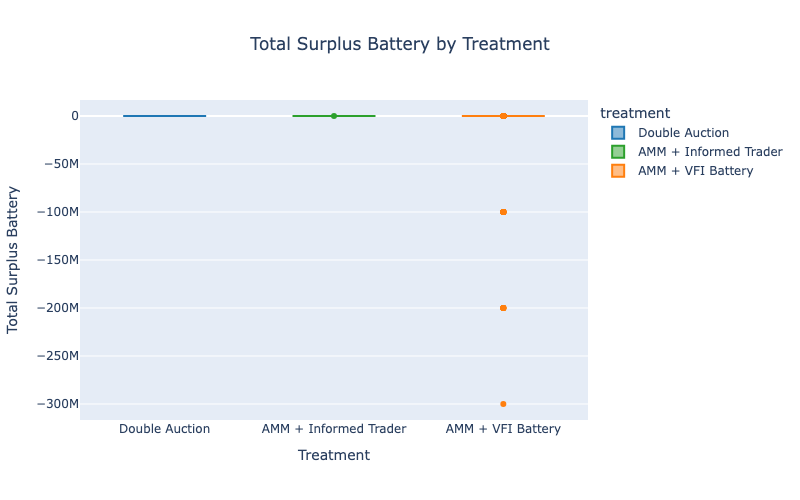
\includegraphics[width=1\linewidth]{images/battery_surplus.png}
    \caption{Boxplot of Battery Surplus by Treatment}
    \label{fig:b_surp}
\end{figure}


\begin{figure}
    \centering
    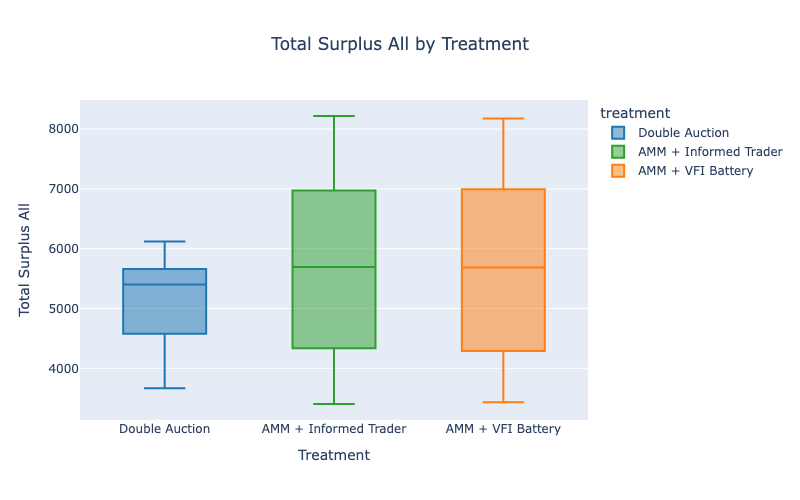
\includegraphics[width=1\linewidth]{images/tot_surp.png}
    \caption{Boxplot of Demand Surplus by Treatment}
    \label{fig:t_surp}
\end{figure}

To address the extreme values observed in the AMM + VFI Battery treatment, we remove outlier rows identified through the interquartile range (IQR) method. Specifically, we calculate the first quartile (Q1) and third quartile (Q3) for \texttt{total\_surplus\_battery}, compute the IQR as $Q3 - Q1$, and define the lower and upper bounds as:
\[
\text{Lower Bound} = Q1 - 1.5 \times \text{IQR}, \quad \text{Upper Bound} = Q3 + 1.5 \times \text{IQR}.
\]
For the AMM + VFI Battery treatment, the summary statistics are:
\begin{itemize}
    \item Q1: $0.00$
    \item Q3: $78.75$
    \item IQR: $78.75$
    \item Lower bound: $-118.12$
    \item Upper bound: $196.87$
\end{itemize}

Any observation falling outside these bounds is classified as an outlier. In total, we detect $76$ outliers out of $480$ observations, corresponding to $15.8\%$ of the sample. These extreme values range from $-3.00 \times 10^{8}$ to $3.08 \times 10^{2}$ and include both highly negative and highly positive surplus values.

When removing these outliers, we also exclude the other treatment observations associated with the same parameter set, ensuring that comparisons across treatments remain balanced. This cleaning step eliminates the disproportionate influence of high-slippage trading episodes in the AMM + VFI Battery, where the battery engages in trades that yield extremely low surpluses for itself but generate correspondingly large surpluses for solar or utility agents.

\newpage
\section{Results}

\subsection{Identification Strategy and Treatment Effects}

Our simulation design produces matched observations across treatments: for each unique parameter configuration, the model is run once under each treatment, where a treatment is defined as a combination of market mechanism and battery strategy. Specifically, we study three treatments: (1) the time-delimited double auction (DA) with a Value Function Iteration (VFI) battery, (2) the Automated Market Maker (AMM) with a VFI battery, and (3) the AMM with an Informed Trader battery. All exogenous simulation parameters—such as battery capacity, initial charge, maximum charge/discharge rates, and solar generation profiles—are held constant across treatments. 

We estimate the following OLS specification:
\[
Y_i = \alpha + \beta \cdot \mathbbm{1}\{\text{Treatment B}_i\} + \mathbf{X}_i'\gamma + \varepsilon_i,
\]
where \(Y_i\) is the surplus outcome of interest, \(\mathbbm{1}\{\text{Treatment B}_i\}\) is an indicator for the treatment of interest, and \(\mathbf{X}_i\) contains the simulation parameters. Because each parameter configuration is observed under both Treatment A and Treatment B, the coefficient \(\beta\) captures the exact average treatment effect (ATE) of switching from Treatment A to Treatment B, conditional on \(\mathbf{X}_i\). 

We perform three pairwise comparisons. First, we compare \textbf{DA + VFI} with \textbf{AMM + VFI} to isolate the effect of the market mechanism while holding the battery strategy fixed. Second, we compare \textbf{AMM + VFI} with\textbf{ AMM + Informed Trader} to isolate the effect of changing the battery strategy while holding the market mechanism fixed. Finally, we compare \textbf{AMM + Informed Trader} directly with \textbf{DA + VFI} to capture the combined effect of simultaneously changing both the market mechanism and the battery strategy. This third comparison is particularly important because it quantifies the net welfare gain from moving directly from the current \textbf{DA + VFI }setup to the proposed\textbf{ AMM + Informed Trader design}, incorporating both mechanism and strategy improvements in a single measure. 


\subsection{Cost of Decentralization: Comparing Social Welfare Between Double Auction and AMM (VFI Battery)}
To ensure a fair comparison of mechanisms, we restrict the sample to AMM runs that used the dynamic programming (VFI) battery—identical to the policy function used in the DA. This isolates the effect of the exchange mechanism itself, holding battery decision-making constant.

The results indicate that the AMM has a large and statistically significant positive effect on \textit{Total Surplus}, increasing it by approximately \(+\$505\) relative to the DA. Rather than revealing a “cost of decentralization,” this specification identifies a substantial welfare \textit{gain} from using an AMM over a Double Auction in this electricity trading environment.

Breaking down the results by agent category:
\begin{itemize}
    \item \textbf{Demand}: The AMM increases demand surplus by about \(+\$276\), significant at the 0.1\% level. This likely reflects greater trade opportunities and slightly lower prices faced by buyers in the continuous AMM market.
    \item \textbf{Solar and Utility}: The AMM raises both solar surplus (\(+\$127\)) and utility surplus (\(+\$232\)), suggesting that sellers also benefit from more continuous price discovery and liquidity provision.
    \item \textbf{Battery}: The AMM decreases battery surplus by roughly \(-\$130\), consistent with earlier discussions of high-slippage trades in thin liquidity states. Although battery surplus is lower, the magnitude of this effect is small relative to the AMM’s overall welfare gain, meaning the battery’s losses are more than offset by the surpluses of other agents.
\end{itemize}

Regarding other covariates:
\begin{itemize}
    \item \(C_{\max}\) is only significant for battery surplus, where it has a positive effect (\(+\$6.39\) per unit increase), as expected from larger operational flexibility.
    \item \(C_{\text{init}}\) and \(q_{b,\max}\) are not statistically significant predictors of surplus for any agent type in this sample.
    \item \(P_{\max}\) and \(\text{std}_{p\max}\) are significant for all surplus measures. Higher \(P_{\max}\) boosts total, demand, and battery surpluses—reflecting cheaper and more abundant electricity—but reduces solar and utility surpluses. This is because high solar output often pushes the clearing price to \(p^* = 0\) in the DA (or near zero in the AMM), reducing seller revenue. Solar variability (\(\text{std}_{p\max}\)) shows a similar pattern: greater variability increases buyer surpluses but reduces seller surpluses.
\end{itemize}

Overall, the regression results suggest that:
\begin{enumerate}
    \item The AMM mechanism generates higher and more evenly distributed surpluses for most agents, even when battery strategies are identical across mechanisms.
    \item The gains to demand, solar, and utility agents more than compensate for the battery’s reduced surplus in the AMM.
    \item Solar output levels and variability have opposing welfare effects for buyers and sellers, consistent with price suppression when renewable generation is abundant.
\end{enumerate}

The high \(R^2\) values for total surplus (\(0.838\)) and demand surplus (\(0.826\)) indicate that the model explains most of the variation in these outcomes, while lower \(R^2\) for battery surplus (\(0.508\)) reflects greater idiosyncratic volatility in battery performance across runs.


\begin{table}[H]
\centering
\caption{DA vs AMM + VFI Trader Analysis}
\label{tab:regression_results}
\begin{tabular}{lccccc}
\hline\hline
 & \textbf{Total Surplus} & \textbf{Demand} & \textbf{Battery} & \textbf{Solar} & \textbf{Utility} \\
\hline
\textbf{AMM} & $505.1680^{***}$ & $276.1376^{***}$ & $-129.9076^{***}$ & $126.6954^{***}$ & $232.2425^{***}$ \\
 & $(35.4162)$ & $(46.4444)$ & $(7.5714)$ & $(15.0123)$ & $(4.4827)$ \\
\textbf{C\_max} & $6.4627$ & $-0.1232$ & $6.3892^{***}$ & $0.5327$ & $-0.3360$ \\
 & $(4.2356)$ & $(5.5545)$ & $(0.9055)$ & $(1.7954)$ & $(0.5361)$ \\
\textbf{C\_init} & $-0.2591$ & $-0.1964$ & $-0.5594$ & $0.5063$ & $-0.0096$ \\
 & $(5.4516)$ & $(7.1492)$ & $(1.1655)$ & $(2.3109)$ & $(0.6900)$ \\
\textbf{q\_b\_max} & $8.1525$ & $1.6143$ & $0.0336$ & $4.9237$ & $1.5809$ \\
 & $(12.6885)$ & $(16.6396)$ & $(2.7126)$ & $(5.3784)$ & $(1.6060)$ \\
\textbf{mean\_pmax} & $168.1487^{***}$ & $210.4532^{***}$ & $13.7470^{***}$ & $-47.1742^{***}$ & $-8.8773^{***}$ \\
 & $(3.6459)$ & $(4.7812)$ & $(0.7794)$ & $(1.5454)$ & $(0.4615)$ \\
\textbf{std\_pmax} & $83.7215^{***}$ & $117.2187^{***}$ & $3.4718^{**}$ & $-31.4852^{***}$ & $-5.4839^{***}$ \\
 & $(5.5352)$ & $(7.2589)$ & $(1.1833)$ & $(2.3463)$ & $(0.7006)$ \\
\hline
R$^2$ & $0.8382$ & $0.8263$ & $0.5083$ & $0.7196$ & $0.8113$ \\
Adj. R$^2$ & $0.8370$ & $0.8250$ & $0.5046$ & $0.7175$ & $0.8098$ \\
Observations & $808$ & $808$ & $808$ & $808$ & $808$ \\
\hline\hline
\end{tabular}
\begin{tablenotes}
\small
\item Note: Standard errors in parentheses. Significance levels: $^{***}$ p$<$0.001, $^{**}$ p$<$0.01, $^{*}$ p$<$0.05.
\end{tablenotes}
\end{table}


\subsubsection{Source of the AMM benefit}

Our analysis indicates that the primary source of the positive surplus generated by the AMM treatment, relative to the Double Auction (DA) treatment, lies in the absence of strict capacity constraints on the AMM’s internal battery. In the current model implementation, the AMM effectively operates as if it has unlimited storage capacity. This allows solar sellers to dispatch \emph{all} of their generation, resulting in the AMM being oversupplied with both energy and corresponding $\Etoken$s.

This oversupply creates a distinctive market dynamic. During evening hours, as the sun sets, solar generation declines and prices begin to rise from near zero toward the utility’s marginal cost. However, because the AMM holds a large reserve of $\Etoken$s, there is a \emph{lag} in this price adjustment: the AMM can continue offering electricity at very low prices for longer than would occur under DA clearing. This prolonged period of low prices leads to higher quantities of demand being served in the AMM scenario. Effectively, the AMM is injecting additional capacity into the market during the transition from day to night.


\begin{figure}[H]
    \centering
    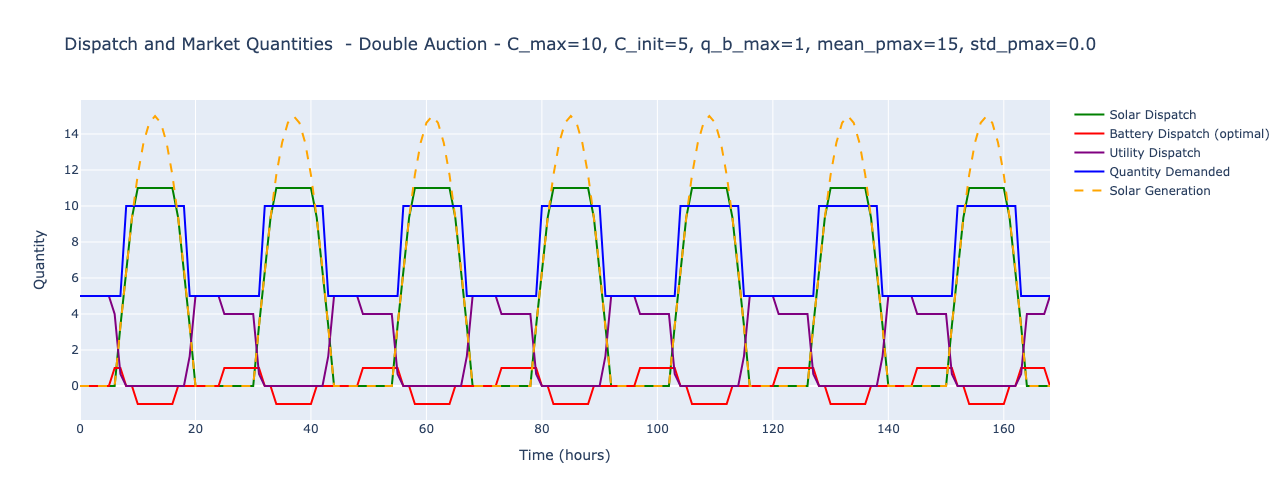
\includegraphics[width=1.15\linewidth]{images/da_excess.png}
    \caption{Excess Solar Double Auction Equilibrium dispatched supply and demand $\eqqdt, \eqqst, \eqqbt, \eqqut$}
    \label{fig:excess_da_dispatch}
\end{figure}

This effect is visible in the dispatch quantities for the DA scenario with parameter values $P_{\max} = 15$, $q_{b,\max} = 1$, $C_{\max} = 10$, $C_{\mathrm{init}} = 5$, and $\text{std}_{p_{\max}} = 0$. In the DA, demand falls sharply as solar generation decreases, and the marginal supplier shifts to the utility. Moreover, not all solar generation is dispatched: battery agents purchase excess supply at zero cost when there is surplus solar, but their charging is constrained by $q_{b,\max}$ and $C_{\max}$, limiting how much can be stored in each period.
\begin{figure}[H]
    \centering
    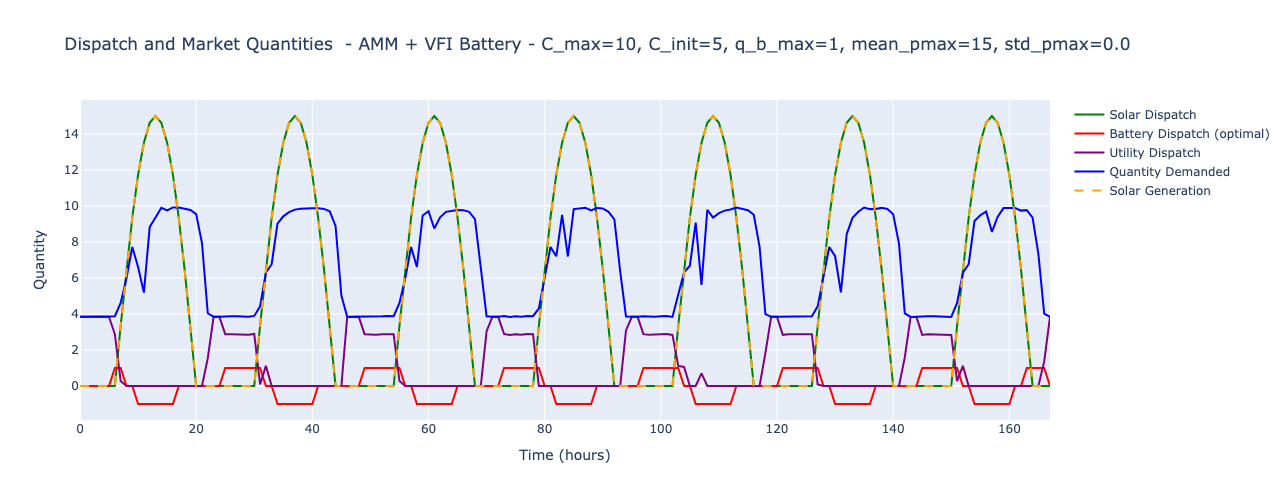
\includegraphics[width=1.15\linewidth]{images/amm_lag.png}
    \caption{Excess Solar AMM final dispatched supply and demand $\eqqdt, \eqqst, \eqqbt, \eqqut$}
    \label{fig:excess_amm_dispatch}
\end{figure}


Furthermore, this lag effect disappears when solar supply is insufficient to meet demand—specifically, when $P_{\max} = 5 < q_{\max} = 10$. In such cases, prices in the AMM remain much closer to the Double Auction equilibrium. The modest price dips that do occur are primarily driven by the AMM’s market-making function, which facilitates trades between buyers and sellers at their respective marginal values or costs, rather than through uniform-price clearing where only one side of the market benefits.

\begin{figure}[H]
    \centering
    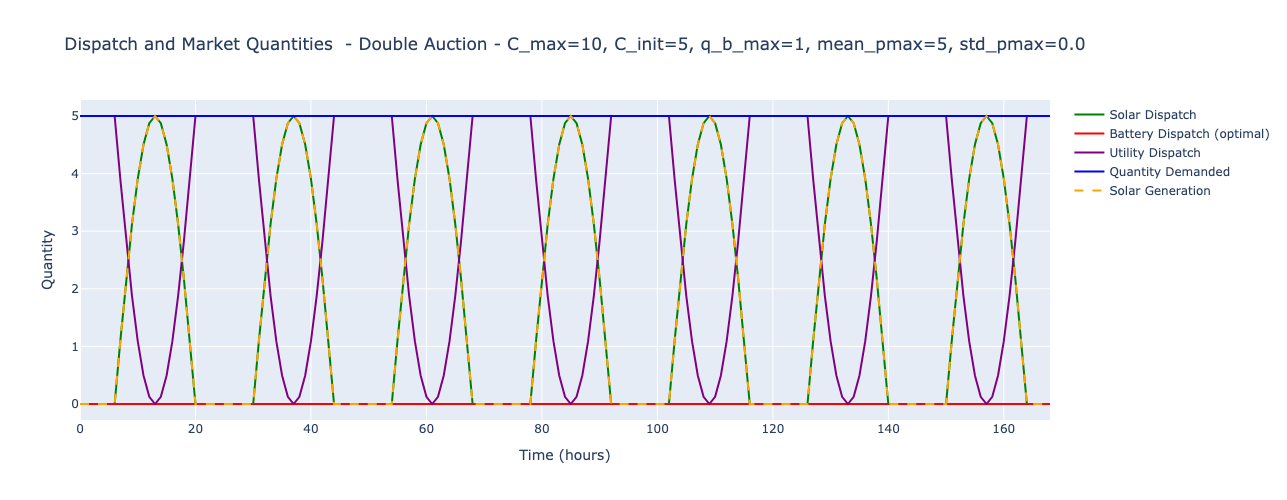
\includegraphics[width=1.15\linewidth]{images/da_low_solar.png}
    \caption{Low solar penetration Double Auction Equilibrium dispatched supply and demand $\eqqdt, \eqqst, \eqqbt, \eqqut$}
    \label{fig:placeholder}
\end{figure}


\begin{figure}[H]
    \centering
    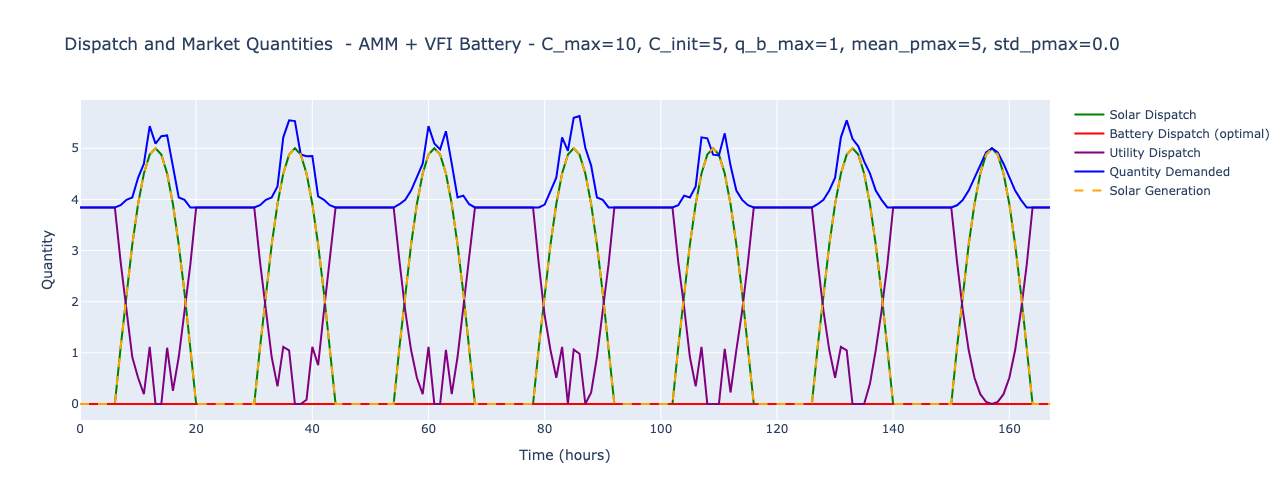
\includegraphics[width=1.15\linewidth]{images/amm_low.png}
    \caption{Low solar penetration AMM final dispatched supply and demand $\eqqdt, \eqqst, \eqqbt, \eqqut$}
    \label{fig:placeholder}
\end{figure}



\subsection{Comparing Social Welfare Between AMM VFI Battery and AMM Informed Trader}

In the previous analysis, we found that AMMs increase surplus for all agent categories except batteries, which can incur substantial negative surplus in certain parameter configurations. To address this, we introduced the \textit{Informed Trader Battery}, a simpler and more targeted trading strategy. This battery observes the expected price differential between the current and next period and executes trades that reduce that differential. The strategy is analogous to how informed traders operate in financial markets when interacting with market makers: they trade based on anticipated price movements rather than purely on optimization over all $T$ periods.

Here, we restrict the dataset to AMM-only runs and compare outcomes for the \textit{Informed Trader} battery relative to the \textit{VFI Battery} benchmark. The coefficient on \textit{Informed Trader} in the \textit{Total Surplus} regression is positive (\(+14.63\)) but statistically insignificant. This suggests that introducing informed trader behavior into the battery does not meaningfully change aggregate welfare compared to the VFI battery. Importantly, this is not a negative result: it implies that the gains from the AMM mechanism remain intact under the informed trader approach, while potentially altering the distribution of surplus across agents.

The key finding is that the informed trader battery achieves a large and statistically significant increase in \textit{Battery Surplus} (\(+210.25\)), indicating that this strategy substantially improves battery profitability compared to the VFI battery. This gain comes without an efficiency loss in total surplus, meaning the informed trader strategy can be adopted without harming the overall system.

However, the results also show statistically significant negative coefficients for demand (\(-136.93\)), solar (\(-43.01\)), and utility (\(-15.68\)) surpluses. This is consistent with the idea that informed traders profit by trading against “noise traders” (agents making trades for exogenous reasons). By anticipating future prices, the battery is able to capture value that would otherwise accrue to other agents, effectively transferring surplus from these groups to itself.

Regarding other covariates, both $C_{\max}$ and $q_{b,\max}$ are significant in the battery surplus model, with positive coefficients. This aligns with economic intuition: larger maximum state of charge and greater per-period charge/discharge capacity enhance the informed trader’s ability to perform intertemporal arbitrage. Initial charge ($C_{\text{init}}$) is also weakly significant for battery surplus, suggesting some influence from starting conditions. The $P_{\max}$ and $\text{std}_{p\max}$ variables follow the same sign patterns as in the previous analysis—positively affecting buyer surplus (demand and battery) while reducing seller surplus (solar and utility) through price suppression effects when renewable generation is abundant or volatile.

Overall, the results indicate that:
\begin{enumerate}
    \item The informed trader battery dramatically improves its own profitability without reducing total surplus in the AMM environment.
    \item These gains come at the expense of other market participants, suggesting a redistribution rather than a net efficiency change.
    \item Larger battery capacity and operational flexibility amplify the informed trader’s advantage.
\end{enumerate}

From a policy or mechanism design perspective, this raises an important trade-off: allowing informed strategies can enhance profitability for certain participants, but may redistribute surplus away from others. Whether such redistribution is desirable depends on broader objectives, such as fairness, investment incentives, and market stability.

\begin{table}[H]
\centering
\caption{AMM Analysis: Informed Trader vs VFI Battery}
\label{tab:amm_regression_results}
\begin{tabular}{lccccc}
\hline\hline
 & \textbf{Total Surplus} & \textbf{Demand} & \textbf{Battery} & \textbf{Solar} & \textbf{Utility} \\
\hline
\textbf{Informed Trader} & $14.6342$ & $-136.9288^{***}$ & $210.2525^{***}$ & $-43.0079^{***}$ & $-15.6817^{***}$ \\
 & $(8.0429)$ & $(6.8067)$ & $(6.2036)$ & $(4.6118)$ & $(1.2538)$ \\
\textbf{C\_max} & $0.8930$ & $-3.3098^{***}$ & $4.0751^{***}$ & $0.6930$ & $-0.5653^{***}$ \\
 & $(0.9619)$ & $(0.8140)$ & $(0.7419)$ & $(0.5515)$ & $(0.1499)$ \\
\textbf{C\_init} & $2.3426$ & $0.4950$ & $2.0604^{*}$ & $0.2403$ & $-0.4532^{*}$ \\
 & $(1.2381)$ & $(1.0478)$ & $(0.9549)$ & $(0.7099)$ & $(0.1930)$ \\
\textbf{q\_b\_max} & $0.2258$ & $-17.5621^{***}$ & $9.4693^{***}$ & $7.2600^{***}$ & $1.0587^{*}$ \\
 & $(2.8815)$ & $(2.4386)$ & $(2.2226)$ & $(1.6523)$ & $(0.4492)$ \\
\textbf{mean\_pmax} & $222.4988^{***}$ & $275.9766^{***}$ & $0.5556$ & $-36.7468^{***}$ & $-17.2866^{***}$ \\
 & $(0.8280)$ & $(0.7007)$ & $(0.6386)$ & $(0.4748)$ & $(0.1291)$ \\
\textbf{std\_pmax} & $139.5908^{***}$ & $195.9624^{***}$ & $-9.3897^{***}$ & $-36.4232^{***}$ & $-10.5587^{***}$ \\
 & $(1.2570)$ & $(1.0638)$ & $(0.9696)$ & $(0.7208)$ & $(0.1960)$ \\
\hline
R$^2$ & $0.9946$ & $0.9977$ & $0.6300$ & $0.9532$ & $0.9785$ \\
Adj. R$^2$ & $0.9946$ & $0.9976$ & $0.6272$ & $0.9529$ & $0.9784$ \\
Observations & $808$ & $808$ & $808$ & $808$ & $808$ \\
\hline\hline
\end{tabular}
\begin{tablenotes}
\small
\item Note: Standard errors in parentheses. Reference category: VFI Battery. Significance levels: $^{***}$ p$<$0.001, $^{**}$ p$<$0.01, $^{*}$ p$<$0.05.
\end{tablenotes}
\end{table}

\subsection{Simple Demonstration of Informed Trader Behavior}

In the figure below, we can see that the informed trader behavior is very similar to the VFI optimized dynamic programming trader wiht the slight difference being that it does most of it's trading in spurts of short intervals during the evening. Since the informed trader expects prices to rise after sunset at hour 20, it buys tokens in the prior periods, and arbitrages some of the price stickyness that is introduced by the AMM battery, it then proceeds to sell as soon as prices settle to the night time. The agent repeats this behavior accross all the days of the week.  

\begin{figure}[H]
    \centering
    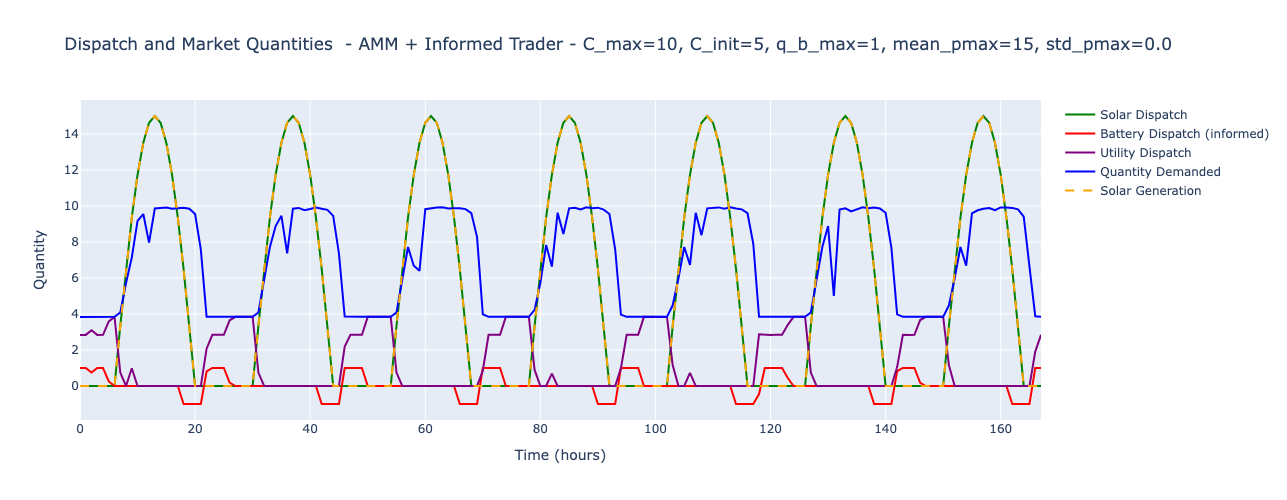
\includegraphics[width=1\linewidth]{images/inf_trader.png}
    \caption{Excess Solar, Informed Trader equilibrium dispatch}
    \label{fig:placeholder}
\end{figure}


\subsection{Comparing Social Welfare Between AMM Informed Trader and Double Auction}

Finally, we compare welfare outcomes between the Double Auction (DA) mechanism and the AMM with the Informed Trader battery. Similar to the earlier comparison with the VFI battery, we find that the AMM has a statistically significant positive effect on total surplus (\(519.80^{***}\)). This estimate is slightly higher than the corresponding effect in the AMM–VFI comparison, but the difference is within the margin of error and therefore not meaningfully different in magnitude.

A key distinction from the VFI battery comparison is that the AMM with an informed trader strategy yields a statistically significant \emph{positive} effect on battery surplus (\(+80.35^{***}\)). In other words, the informed trader battery not only avoids the negative surplus outcomes observed for the VFI battery in some configurations, but it also generates net positive gains for the battery agent. Moreover, the AMM treatment is associated with positive and statistically significant effects on the surpluses of \emph{all} agent categories—demand, solar, utility, and battery—indicating that, in this configuration, every participant type benefits from the AMM relative to the DA.

As in earlier regressions, both \(\text{mean\_}P_{\max}\) and \(\text{std\_}P_{\max}\) remain significant predictors of surplus outcomes. Higher average maximum solar generation (\(\text{mean\_}P_{\max}\)) increases total surplus and buyer surpluses (demand and battery) while reducing seller surpluses (solar and utility) due to price suppression effects when renewable generation is abundant. Variability in solar generation (\(\text{std\_}P_{\max}\)) has similar directional effects, though the battery surplus effect is negative here and statistically insignificant, suggesting that volatility in generation does not strongly affect battery profits under the informed trader strategy.

Among the battery-specific parameters, \(C_{\max}\) and \(q_{b,\max}\) are again positively and significantly associated with battery surplus, consistent with the idea that greater storage capacity and larger allowable per-period trades enable more effective intertemporal arbitrage.

Overall, these results suggest that:
\begin{enumerate}
    \item The AMM with an informed trader battery outperforms the DA in total surplus while delivering gains to \emph{all} agent types.
    \item Unlike the VFI battery, the informed trader battery produces positive surplus for itself without reducing the surpluses of other participants.
    \item Battery capacity and operational flexibility remain important drivers of battery profitability in the AMM environment.
\end{enumerate}

From a market design perspective, these findings imply that informed trading in AMMs can be welfare-enhancing across the board, potentially alleviating the distributional concerns observed with more complex optimization-based battery strategies.


\begin{table}[H]
\centering
\caption{DA vs AMM + Informed Trader Analysis}
\label{tab:da_informed_regression_results}
\begin{tabular}{lccccc}
\hline\hline
 & \textbf{Total Surplus} & \textbf{Demand} & \textbf{Battery} & \textbf{Solar} & \textbf{Utility}\\
\hline
\textbf{AMM} & $519.8021^{***}$ & $139.2089^{**}$ & $80.3450^{***}$ & $83.6875^{***}$ & $216.5608^{***}$ \\
 & $(35.3491)$ & $(49.2519)$ & $(9.8681)$ & $(14.3468)$ & $(4.1332)$ \\
\textbf{C\_max} & $5.6931$ & $-2.0606$ & $8.3205^{***}$ & $-0.3376$ & $-0.2293$ \\
 & $(4.2275)$ & $(5.8902)$ & $(1.1802)$ & $(1.7158)$ & $(0.4943)$ \\
\textbf{C\_init} & $1.7202$ & $0.2819$ & $1.8430$ & $0.0389$ & $-0.4436$ \\
 & $(5.4413)$ & $(7.5814)$ & $(1.5190)$ & $(2.2084)$ & $(0.6362)$ \\
\textbf{q\_b\_max} & $7.3720$ & $-16.1229$ & $23.8893^{***}$ & $0.1279$ & $-0.5222$ \\
 & $(12.6644)$ & $(17.6454)$ & $(3.5354)$ & $(5.1400)$ & $(1.4808)$ \\
\textbf{mean\_pmax} & $167.5127^{***}$ & $216.6787^{***}$ & $10.3396^{***}$ & $-51.0963^{***}$ & $-8.4093^{***}$ \\
 & $(3.6390)$ & $(5.0702)$ & $(1.0159)$ & $(1.4769)$ & $(0.4255)$ \\
\textbf{std\_pmax} & $84.8602^{***}$ & $121.8398^{***}$ & $-2.9583$ & $-28.9464^{***}$ & $-5.0748^{***}$ \\
 & $(5.5247)$ & $(7.6976)$ & $(1.5423)$ & $(2.2423)$ & $(0.6460)$ \\
\hline
R$^2$ & $0.8390$ & $0.8179$ & $0.2704$ & $0.7484$ & $0.8150$ \\
Adj. R$^2$ & $0.8378$ & $0.8165$ & $0.2650$ & $0.7465$ & $0.8136$ \\
Observations & $808$ & $808$ & $808$ & $808$ & $808$ \\
\hline\hline
\end{tabular}
\begin{tablenotes}
\small
\item Note: Standard errors in parentheses. Reference category: Double Auction. Significance levels: $^{***}$ p$<$0.001, $^{**}$ p$<$0.01, $^{*}$ p$<$0.05.
\end{tablenotes}
\end{table}


\section{Conclusion}

Our results demonstrate that, within the modeled environment, the AMM mechanism consistently delivers higher total social welfare than the time-delimited double auction, even when battery strategies and parameter configurations vary. While the VFI-optimized battery often produces negative surplus under the AMM, these losses are more than offset by gains to demand, solar, and utility agents. The introduction of the informed trader battery eliminates the negative battery surplus without reducing overall welfare, suggesting that targeted strategy adjustments can improve agent outcomes without sacrificing efficiency.

These findings imply that the \emph{cost of decentralization}—measured as welfare loss from adopting an AMM over a double auction—can, in certain contexts, be negative, meaning decentralization may yield net welfare gains. However, the AMM's advantage partly arises from implicit capacity flexibility not present in the double auction, a factor that may not generalize to real-world deployments. Future work should examine the effects of introducing strict capacity constraints and more heterogeneous trading behavior to better approximate operational realities.




\section{Data and Code Availability Statement}

The GitHub repository containing the agent-based model code as well as the dynamic programming implementation is available at  
\href{https://github.com/nalinbhatt/MA_thesis.git}{GitHub Repo}.  

The cleaned and summarized model output is located in the \texttt{Data Analysis} folder and can be accessed  
\href{https://github.com/nalinbhatt/MA_thesis/blob/main/Data%20Analysis/da_amm_combined.csv}{here}.  
All relevant analysis, including visualizations, can be conducted and found  in the  
\href{https://github.com/nalinbhatt/MA_thesis/blob/main/Data%20Analysis/data_analysis.ipynb}{\texttt{data\_analysis.ipynb}} notebook.  

The code for running the parameter-sweep Double Auction Value Function Iteration simulations is located in  
\href{https://github.com/nalinbhatt/MA_thesis/blob/main/DA%20Model/vfi_simulations.py}{\texttt{vfi\_simulations.py}}.  

Finally, the code for the agent-based simulation parameter sweep can be found in 
\href{https://github.com/nalinbhatt/MA_thesis/blob/main/ABM%20Model/multi_simulation_runner.py}{\texttt{multi\_simulation\_runner.py}}.


\newpage

\part*{Appendix}
\fancyhead[L]{\textsc{Appendix}}
%\setcounter{page}{1}
\setcounter{section}{0}

\section{Automated Market Maker Trading Example}

This section provides two illustrative examples of how an Automated Market Maker (AMM) facilitates electricity trades using a constant product pricing function. These examples demonstrate a prosumer selling electricity to the AMM, and a consumer purchasing electricity from it.

\subsection{Prosumer Sells Electricity to AMM}\label{swap_example1}

We assume the AMM operates using the constant product formula:
\[
M_{\text{token}} \times E_{\text{token}} = k,
\]
where \(M_{\text{token}}\) is the money reserve (e.g., dollars), and \(E_{\text{token}}\) is the electricity reserve (e.g., kWh). Initially, \(M_{\text{token}} = 10\) and \(E_{\text{token}} = 5\), so \(k = 50\).

Suppose a prosumer wants to sell \(1\) unit of energy to the AMM. After the trade, the new electricity reserve becomes \(E_{\text{token}} + 1 = 6\), and we solve for the corresponding decrease in the money reserve \(\Delta_{M_{\text{token}}}\) using:
\[
(M_{\text{token}} - \Delta_{M_{\text{token}}})(E_{\text{token}} + 1) = k,
\]
\[
(10 - \Delta_{M_{\text{token}}})(6) = 50 \Rightarrow \Delta_{M_{\text{token}}} = 1.67.
\]

\begin{table}[H]
\centering
\caption{Prosumer Trade with AMM}
\begin{tabular}{c|l|c}
\textbf{Symbol} & \textbf{Description} & \textbf{Value} \\
\hline
\(M_{\text{token}}\) & Money reserves (before trade) & 10 \\
\(E_{\text{token}}\) & Electricity reserves (before trade) & 5 \\
\(\Delta_{E_{\text{token}}}\) & Electricity sold by prosumer & 1 \\
\(\Delta_{M_{\text{token}}}\) & Money received by prosumer & 1.67 \\
\(k\) & Constant product \(M \times E\) & 50 \\
\end{tabular}
\end{table}

\begin{figure}[H]
    \centering
    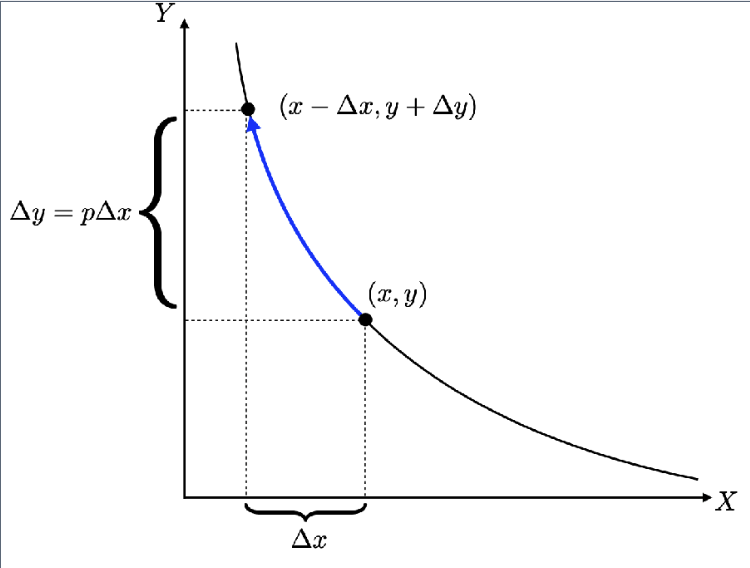
\includegraphics[width=0.4\textwidth]{images/edited_amm_swap.png}
    \caption{Illustration of prosumer-initiated swap with AMM. Source: \cite{aoyagi_coexisting_nodate}}
\end{figure}

\subsection{Consumer Buys Electricity from AMM}\label{swap_example2}

Now consider a consumer purchasing \(1\) unit of electricity from the AMM. A transaction fee \(t = 0.01\) applies to each trade. The AMM’s reserves before the trade remain:
\[
M_{\text{token}} = 10, \quad E_{\text{token}} = 5, \quad k = 50.
\]

The post-trade electricity reserve becomes \(E_{\text{token}} - 1 = 4\), and the equation with the fee-adjusted payment becomes:
\[
(M_{\text{token}} + (1 - t)\Delta_{M_{\text{token}}})(E_{\text{token}} - 1) = k,
\]
\[
(10 + 0.99\Delta_{M_{\text{token}}})(4) = 50 \Rightarrow \Delta_{M_{\text{token}}} = 2.52.
\]

\subsection{Liquidity Provision in AMMs}\label{lp_math}

\subsubsection*{1. Mechanism}

Consider a constant product AMM (e.g., Uniswap v2), where the product of reserves remains constant:
\[
M \times E = k,
\]
where \(M\) is the reserve of the monetary token (e.g., dollars), and \(E\) is the reserve of the electricity token (e.g., kilowatt-hours). A liquidity provider contributes an initial amount \((M_0, E_0)\) such that:
\[
\frac{M_0}{M} = \frac{E_0}{E},
\]
ensuring the pool remains balanced and the price unchanged.

Upon deposit, the provider receives a number of LP tokens proportional to:
\[
\text{LP}_{\text{issued}} = \frac{M_0}{M_{\text{total}}} \times \text{LP}_{\text{total}},
\]
where \(\text{LP}_{\text{total}}\) is the total supply of LP tokens. If the pool is empty, the provider typically receives a fixed number of LP tokens equal to the geometric mean:
\[
\text{LP}_{\text{issued}} = \sqrt{M_0 \cdot E_0}.
\]

\subsubsection*{2. Earning Fees}

When a user executes a trade (e.g., sells electricity to the AMM), they pay a fee \(t\) (e.g., \(t = 0.003\) or 0.3\%) on the input token. This fee remains in the pool, increasing the total reserves. Since LP tokens represent proportional claims on the reserves, LPs benefit from this fee accumulation over time.

Thus, liquidity provision allows agents to passively earn yield through transaction fees, even in the absence of active trading.


\begin{table}[H]
\centering
\caption{Consumer Trade with AMM}
\begin{tabular}{c|l|c}
\textbf{Symbol} & \textbf{Description} & \textbf{Value} \\
\hline
\(M_{\text{token}}\) & Money reserves (before trade) & 10 \\
\(E_{\text{token}}\) & Electricity reserves (before trade) & 5 \\
\(\Delta_{E_{\text{token}}}\) & Electricity bought by consumer & 1 \\
\(\Delta_{M_{\text{token}}}\) & Money paid by consumer & 2.52 \\
\(t\) & Transaction fee & 0.01 \\
\(k\) & Constant product \(M \times E\) & 50 \\
\end{tabular}
\end{table}

\section{Result Plots}

\begin{figure}[H]
    \centering
    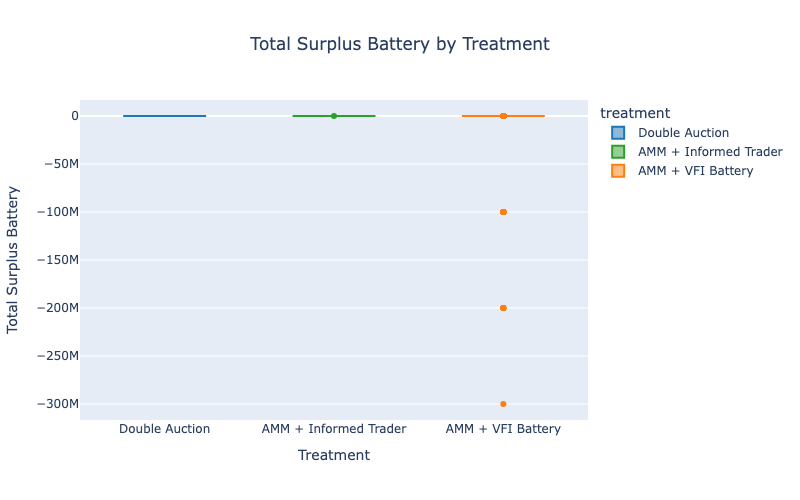
\includegraphics[width=0.75\linewidth]{images/solar_surp.png}
    \caption{Boxplot of Solar Surplus by Treatment}
    \label{fig:s_surp}
\end{figure}

\begin{figure}[H]
    \centering
    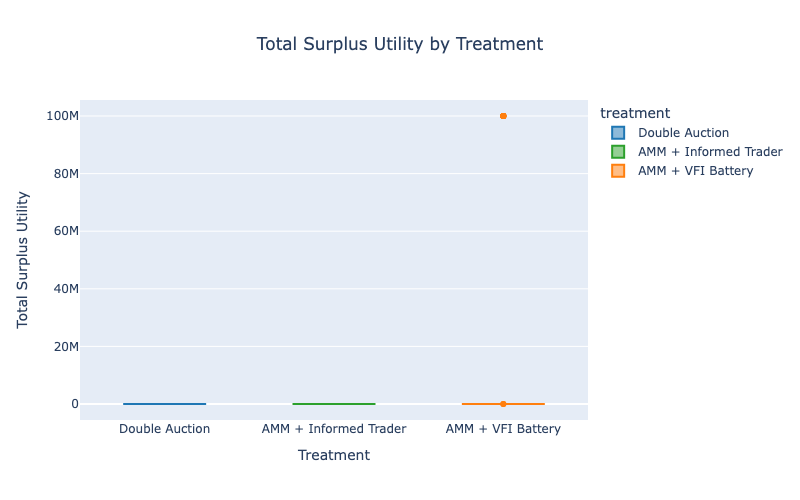
\includegraphics[width=0.75\linewidth]{images/util_surp.png}
    \caption{Boxplot of Utility Surplus by Treatment}
    \label{fig:u_surp}
\end{figure}

\begin{figure}[H]
    \centering
    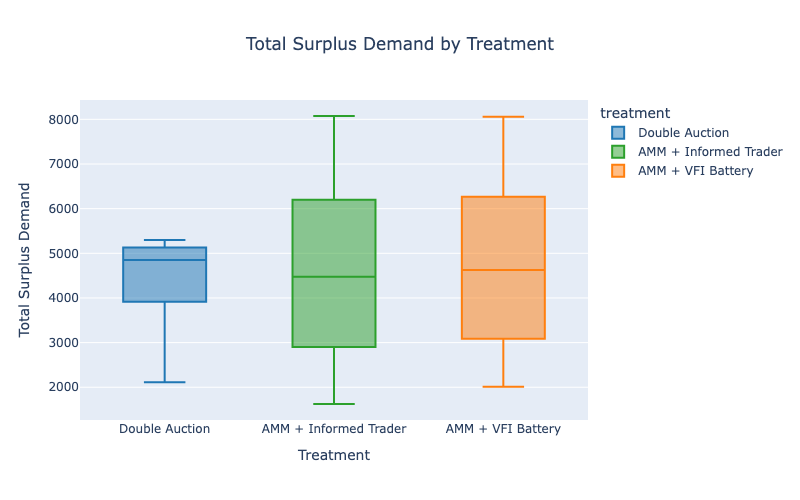
\includegraphics[width=0.75\linewidth]{images/d_surp.png}
    \caption{Boxplot of Demand Surplus by Treatment}
    \label{fig:d_surp}
\end{figure}


\begin{sidewaystable}
%\begin{table}[htbp]
\centering
\caption{Summary Welfare Statistics by Treatment}
\label{tab:summary_statistics}
\small
\begin{tabular}{llrrrrrrrr}
\toprule
\textbf{Total Surplus} & \textbf{Treatment} & \textbf{Count} & \textbf{Mean} & \textbf{Std} & \textbf{Min} & \textbf{25\%} & \textbf{50\%} & \textbf{75\%} & \textbf{Max} \\
\midrule

\multirow{1}{*}{\textbf{Battery}} 
& AMM + Informed Trader & 480 & 262.33 & 137.95 & 6.15 & 183.44 & 244.03 & 358.49 & 632.99 \\
& AMM + VFI Battery      & 480 & -7083592.68 & 32820369.64 & -3.00e+08 & 0.00 & 0.00 & 78.75 & 307.77 \\
& Double Auction         & 480 & 212.76 & 214.55 & 0.00 & 0.00 & 175.00 & 350.00 & 700.00 \\
\midrule

\multirow{1}{*}{\textbf{Solar}} 
& AMM + Informed Trader & 480 & 603.49 & 305.56 & 34.61 & 353.04 & 614.64 & 904.74 & 1028.23 \\
& AMM + VFI Battery      & 480 & 5000966.91 & 28462739.78 & 42.12 & 551.97 & 762.89 & 932.04 & 3.00e+08 \\
& Double Auction         & 480 & 506.65 & 455.45 & 118.43 & 207.63 & 343.54 & 563.12 & 1553.17 \\
\midrule

\multirow{1}{*}{\textbf{Utility}} 
& AMM + Informed Trader & 480 & 201.23 & 114.93 & 10.23 & 98.74 & 201.85 & 307.87 & 380.51 \\
& AMM + VFI Battery      & 480 & 2083555.87 & 14297490.29 & 11.05 & 102.24 & 219.11 & 358.25 & 1.00e+08 \\
& Double Auction         & 480 & 0.00 & 0.00 & 0.00 & 0.00 & 0.00 & 0.00 & 0.00 \\
\midrule

\multirow{1}{*}{\textbf{Demand}} 
& AMM + Informed Trader & 480 & 4630.62 & 1985.92 & 1624.96 & 3056.65 & 4474.17 & 6191.15 & 8074.86 \\
& AMM + VFI Battery      & 480 & 4760.97 & 1892.50 & 2011.47 & 3299.18 & 4628.05 & 6234.51 & 8058.17 \\
& Double Auction         & 480 & 4395.78 & 1040.67 & 2112.50 & 4193.75 & 4850.00 & 5084.38 & 5300.00 \\
\midrule

\multirow{1}{*}{\textbf{All}} 
& AMM + Informed Trader & 480 & 5697.67 & 1519.52 & 3403.07 & 4518.00 & 5691.92 & 6970.46 & 8218.48 \\
& AMM + VFI Battery      & 480 & 5691.09 & 1524.12 & 3433.57 & 4477.33 & 5685.67 & 6992.32 & 8177.87 \\
& Double Auction         & 480 & 5115.19 & 750.68 & 3665.67 & 4756.87 & 5402.10 & 5661.53 & 6118.43 \\
\bottomrule
\end{tabular}
%\end{table}
\end{sidewaystable}



\newpage

\part*{References}
\fancyhead[L]{\textsc{References}}

\setcounter{page}{1}
\label{references}
\printbibliography[heading=none]




\end{document}








